\documentclass[conference]{IEEEtran}
\usepackage[utf8]{inputenc}
\usepackage[T1]{fontenc}
\usepackage[spanish,es-nodecimaldot]{babel}
\usepackage{amsmath,amssymb}
\usepackage{newtxtext,newtxmath} % Tipografía estándar IEEE (Times)
\usepackage{graphicx,booktabs,array,url,stfloats,microtype}
\usepackage[hidelinks]{hyperref}
\hypersetup{pdftitle={Evaluación Comparativa de Tres Arquitecturas CNN para Clasificación de Lesiones Cutáneas Pigmentadas mediante Dermatoscopia (HAM10000)},pdfauthor={Grupo 9 - UNSAAC}}
\graphicspath{{img/}}

\title{Evaluaci\'on Comparativa de Tres Arquitecturas CNN para Clasificaci\'on de Lesiones Cut\'aneas Pigmentadas mediante Dermatoscopia (HAM10000)}

\author{
\IEEEauthorblockN{
Noe Franklin Choquenaira Quispe\IEEEauthorrefmark{1},
Yeni Ruth Porroa Sivana\IEEEauthorrefmark{2},
Jean Franco Colque Galindo\IEEEauthorrefmark{3}
}
\IEEEauthorblockA{
Grupo N.\ 9 -- Visi\'on por Computador (2026-II) $\cdot$ Docente: Mg. Hans Harley Ccacyahuillca Bejar\\
Escuela Profesional de Ingenier\'ia Inform\'atica y de Sistemas, Universidad Nacional de San Antonio Abad del Cusco, Per\'u\\
C\'odigos: \IEEEauthorrefmark{1}133962, \IEEEauthorrefmark{2}120893, \IEEEauthorrefmark{3}193109
}
}

\begin{document}
\maketitle

\begin{abstract}
La clasificaci\'on autom\'atica de lesiones dermatosc\'opicas enfrenta tres retos centrales: desbalance severo entre categor\'ias, dependencia entre m\'ultiples tomas de una misma lesi\'on y restricciones de c\'omputo. Se ejecuta y eval\'ua un estudio comparativo reproducible entre tres redes neuronales convolucionales (CNN) compactas---\textbf{ResNet-18}, \textbf{EfficientNet-B0} y \textbf{MobileNetV3-Small}---mediante transferencia de aprendizaje sobre \textbf{HAM10000}. La auditor\'ia verifica 10\,015 im\'agenes RGB (7\,470 lesiones, siete clases), detecta dos pares binarios id\'enticos por SHA-256 en \texttt{nv} y cero pares casi id\'enticos ($\mathrm{RMSE}<4.5$) entre lesiones distintas en verificaci\'on de sesi\'on, construyendo mediante \texttt{StratifiedGroupKFold} una partici\'on fija libre de fuga (7\,009 entrenamiento, 1\,503 validaci\'on, 1\,503 prueba). Bajo protocolo homog\'eneo en GPU NVIDIA GTX~1650 (4~GiB, PyTorch~2.11.0+cu128, FP32, lote~8, \texttt{num\_workers=4}, semilla~42), \textbf{ResNet-18} ofrece el mejor compromiso observado en este protocolo y GPU sobre prueba limpia: Accuracy de $0.8031$, Macro~Prec.\ de $0.6591$, Macro~F1 de $0.6786$, exactitud balanceada de $0.7174$, AUC~OVR de $0.9596$, sensibilidad de melanoma de $0.6012$ y latencia mediana \texttt{forward()} (\texttt{batch=1}) de $7.22$~ms ($434.2$~MiB de VRAM). \textbf{EfficientNet-B0} alcanza un Macro~F1 muy pr\'oximo ($0.6778$; $\Delta=0.00084$, sin superioridad ni equivalencia estad\'istica), lidera en Macro~Prec.\ ($0.6741$) y sensibilidad limpia de melanoma ($0.6607$), pero con $24.60$~ms de latencia, $805.7$~MiB de VRAM y la mayor ca\'ida ante ruido gaussiano \texttt{noise\_005} ($\Delta\mathrm{F1}=+0.5577$). \textbf{MobileNetV3-Small} consume menor memoria ($211.8$~MiB) con menor Macro~F1 ($0.5700$, Macro~Prec.\ $0.6474$) y $22.40$~ms en limpio. El filtrado espacial previo \texttt{gaussian\_1} sobre \texttt{noise\_005} aporta entre $+0.14$ y $+0.33$ puntos de Macro~F1 como mitigaci\'on parcial, elevando el Macro~F1 de ResNet-18 a $0.5104$ y su Recall de melanoma a $0.6905$, aunque reduciendo su precisi\'on en esa clase de $0.5233$ a $0.3648$ ($92 \to 202$ falsos positivos). Este trabajo es estrictamente acad\'emico y no constituye una herramienta de diagn\'ostico cl\'inico.
\end{abstract}

\begin{IEEEkeywords}
HAM10000, clasificaci\'on dermatosc\'opica, CNN, transferencia de aprendizaje, partici\'on por grupos, macro F1, robustez, reproducibilidad.
\end{IEEEkeywords}

\section{Introducci\'on}
El an\'alisis automatizado de im\'agenes dermatosc\'opicas busca apoyar el cribado temprano de neoplasias cut\'aneas pigmentadas y no pigmentadas, especialmente el melanoma frente a lesiones benignas frecuentes \cite{tschandl2018,codella2019}. Sin embargo, construir estudios comparativos v\'alidos entre arquitecturas de aprendizaje profundo exige controlar factores que suelen distorsionar las m\'etricas reportadas en la literatura acad\'emica: la fuga de informaci\'on entre particiones, el sesgo introducido por clases mayoritarias y la comparaci\'on desigual de hardware o preprocesamiento.

El conjunto HAM10000 (\textit{Human Against Machine with 10000 training images}) presenta una asimetr\'ia pronunciada: la clase \texttt{nv} (nevus melanoc\'itico) concentra 6\,705 de las 10\,015 im\'agenes (66.95\%), frente a apenas 115 im\'agenes en \texttt{df} (dermatofibroma, 1.15\%), lo que representa una raz\'on de desbalance de $58.3:1$ \cite{tschandl2018}. En ese escenario, la exactitud global (\textit{Accuracy}) puede superar el 66\% con un clasificador trivial que prediga siempre la clase mayoritaria. Adicionalmente, m\'ultiples tomas de una misma lesi\'on f\'isica a distintas magnificaciones o \'angulos implican que una partici\'on aleatoria por imagen distribuye fotograf\'ias correlacionadas entre entrenamiento y prueba, inflando artificialmente el rendimiento aparente.

En este art\'iculo se dise\~na, implementa y eval\'ua experimentalmente un protocolo reproducible para contrastar tres arquitecturas CNN de distinta familia estructural---\textbf{ResNet-18} \cite{he2016}, \textbf{EfficientNet-B0} \cite{tan2019} y \textbf{MobileNetV3-Small} \cite{howard2019}---sobre la tarea unificada de clasificaci\'on multiclase de siete categor\'ias en HAM10000. Las contribuciones principales del trabajo son:
\begin{enumerate}
\item \textbf{Auditor\'ia criptogr\'afica y perceptual del dataset:} comprobaci\'on \'integra de 10\,015 im\'agenes y metadatos, consolidaci\'on de los lotes \texttt{part\_1} y \texttt{part\_2}, detecci\'on de duplicados binarios por SHA-256 y verificaci\'on de casi-duplicados entre lesiones distintas.
\item \textbf{Partici\'on fija sin fuga y artefactos auditables:} generaci\'on de un manifiesto reproducible ($\sim$70\%/15\%/15\%) y exportaci\'on de la estructura jer\'arquica \texttt{train/val/test} por clase, con estad\'isticas calculadas estrictamente sobre entrenamiento.
\item \textbf{Protocolo homog\'eneo y ejecutado en GPU local:} entrenamiento determinista completo sobre GTX~1650 (4~GiB) tras comprobaci\'on previa de sesi\'on con \texttt{num\_workers=4}, selecci\'on por Macro~F1 en \texttt{val}, checkpoints at\'omicos y medici\'on sincronizada de latencia \texttt{forward()} y VRAM.
\item \textbf{Evaluaci\'on comparativa integral y mitigaci\'on parcial:} cuantificaci\'on en \texttt{test} limpio ($n=1\,503$), an\'alisis de degradaci\'on bajo cinco perturbaciones deterministas y evaluaci\'on de filtrado espacial previo (\texttt{median\_3} y \texttt{gaussian\_1}) frente a \texttt{noise\_005}, registrando tanto la recuperaci\'on de sensibilidad como el intercambio en precisi\'on y falsos positivos.
\end{enumerate}

Todos los experimentos de entrenamiento, prueba limpia, sensibilidad al ruido/desenfoque y eficiencia se completaron sobre el protocolo congelado; el despliegue interactivo queda excluido del alcance acad\'emico del proyecto por indicaci\'on docente.

\section{Trabajos Relacionados}
La publicaci\'on de HAM10000 y su integraci\'on en el desaf\'io ISIC~2018 establecieron un marco est\'andar para clasificar siete categor\'ias pigmentadas con verificaci\'on multifuente (histopatolog\'ia, seguimiento digital, consenso experto y microscop\'ia confocal) \cite{tschandl2018,codella2019}. Una lecci\'on central de dicha literatura es la necesidad de agrupar por \texttt{lesion\_id} antes de dividir el conjunto para evitar evaluar sobre vistas repetidas de lesiones presentes en entrenamiento.

En el dise\~no de arquitecturas convolucionales \cite{goodfellow2016}, ResNet introdujo conexiones residuales para mitigar problemas de optimizaci\'on al incrementar profundidad \cite{he2016}. Posteriormente, EfficientNet propuso el escalado compuesto simult\'aneo de profundidad, ancho y resoluci\'on a partir de bloques invertidos con atenci\'on por canal (\textit{Squeeze-and-Excitation}, SE) \cite{tan2019}. Por su parte, MobileNetV3 combin\'o b\'usqueda neuronal orientada a latencia en hardware restringido con bloques invertidos separables en profundidad, m\'odulos SE y no linealidad \textit{hard-swish} \cite{howard2019}.

Cuando la colecci\'on objetivo tiene tama\~no moderado (del orden de $10^4$ im\'agenes), la transferencia de aprendizaje desde representaciones preentrenadas en ImageNet acelera la convergencia frente al entrenamiento desde cero, requiriendo adaptar la cabeza clasificadora y controlar tasas de aprendizaje durante el ajuste fino \cite{pan2010}. Asimismo, en presencia de desbalance severo, Saito y Rehmsmeier mostraron que las m\'etricas globales pueden resultar enga\~nosas si no se eval\'uan por clase junto a curvas de precisi\'on-exhaustividad y sensibilidad de la clase cr\'itica \cite{saito2015}.

A diferencia de estudios que comparan algoritmos modificando simult\'aneamente resoluci\'on, partici\'on o hardware de medici\'on, nuestro estudio fija el mismo manifiesto de partici\'on, la misma transformaci\'on geom\'etrica y el mismo presupuesto de optimizaci\'on para evaluar de manera honesta el compromiso entre calidad diagn\'ostica acad\'emica y costo computacional en una GPU m\'ovil de 4~GiB.

\section{Materiales y M\'etodos}

\subsection{Auditor\'ia del Conjunto HAM10000 y Partici\'on sin Fuga}
El conjunto descargado de Kaggle (\texttt{kmader/skin-cancer-mnist-ham10000}, versi\'on~2) presentaba originalmente carpetas duplicadas por diferencia de may\'usculas y min\'usculas (\texttt{HAM10000\_images\_part\_*} y \texttt{ham10000\_images\_part\_*}). Tras verificar igualdad exacta de CRC y tama\~no en los 10\,015 pares, se depur\'o el archivo eliminando las copias redundantes (reduciendo de 5.199~GiB a 2.706~GiB). Se confirm\'o adem\'as que \texttt{part\_1} (5\,000 im\'agenes) y \texttt{part\_2} (5\,015 im\'agenes) son lotes complementarios de un mismo conjunto con intersecci\'on nula, no particiones ni clases.

La auditor\'ia program\'atica comprob\'o correspondencia exacta entre los 10\,015 JPEG (resoluci\'on nativa $600\times450$ p\'ixeles) y las 10\,015 filas de \texttt{HAM10000\_metadata.csv}, correspondiendo a 7\,470 valores \'unicos de \texttt{lesion\_id}. Mediante huellas SHA-256 se identificaron dos pares de registros binariamente id\'enticos con distinto \texttt{image\_id} (\texttt{ISIC\_0024366}/\texttt{ISIC\_0029861} en \texttt{HAM\_0002300} y \texttt{ISIC\_0024777}/\texttt{ISIC\_0029938} en \texttt{HAM\_0001895}), ambos dentro de la clase \texttt{nv}. Adicionalmente, como comprobaci\'on previa de sesi\'on (sin artefacto independiente persistido en el repositorio), se realiz\'o un barrido por parejas sobre miniaturas RGB $16\times12$ entre todas las muestras con distinto \texttt{lesion\_id}, observando \textbf{cero pares} con $\mathrm{RMSE}<4.5$; ello descarta duplicados triviales a baja resoluci\'on, aunque mantiene abierta la limitaci\'on de similitud perceptual dermatosc\'opica entre lesiones distintas.

Para construir la partici\'on oficial se emple\'o \texttt{StratifiedGroupKFold} con $K=20$ pliegues, mezcla reproducible y semilla 42 \cite{sklearndocs}, agrupando por la uni\'on de \texttt{lesion\_id} y hash SHA-256. Se asignaron los pliegues $0\text{--}2$ a prueba (\texttt{test}), $3\text{--}5$ a validaci\'on (\texttt{val}) y $6\text{--}19$ a entrenamiento (\texttt{train}). Como refleja el Cuadro~\ref{tab:split} y la Fig.~\ref{fig:clases_split}, las siete categor\'ias quedan representadas en los tres subconjuntos sin cruce alguno de lesi\'on, grupo o SHA-256.

\begin{table*}[t]
\centering
\caption{Auditor\'ia comprobada del conjunto HAM10000, partici\'on fija libre de fuga ($\sim$70/15/15) y pesos de clase en entrenamiento.}
\label{tab:split}
\begin{tabular}{llrrrrrrr}\toprule
C\'odigo & Categor\'ia cl\'inica & Im\'agenes & Lesiones & \% Total & Train & Val & Test & Peso $w_c$ \\ \midrule
\texttt{akiec} & Queratosis act\'inica / Bowen & 327 & 228 & 3.27 & 228 & 50 & 49 & 4.3916 \\
\texttt{bcc} & Carcinoma basocelular & 514 & 327 & 5.13 & 359 & 77 & 78 & 2.7891 \\
\texttt{bkl} & Queratosis benigna & 1\,099 & 727 & 10.97 & 769 & 165 & 165 & 1.3021 \\
\texttt{df} & Dermatofibroma & 115 & 73 & 1.15 & 80 & 18 & 17 & 12.5161 \\
\texttt{mel} & Melanoma & 1\,113 & 614 & 11.11 & 779 & 166 & 168 & 1.2853 \\
\texttt{nv} & Nevus melanoc\'itico & 6\,705 & 5\,403 & 66.95 & 4\,694 & 1\,006 & 1\,005 & 0.2133 \\
\texttt{vasc} & Lesi\'on vascular & 142 & 98 & 1.42 & 100 & 21 & 21 & 10.0129 \\ \midrule
\textbf{Total} & \textbf{7 categor\'ias} & \textbf{10\,015} & \textbf{7\,470} & \textbf{100.00} & \textbf{7\,009} & \textbf{1\,503} & \textbf{1\,503} & --- \\
\bottomrule
\end{tabular}
\end{table*}

\begin{figure}[t]
\centering
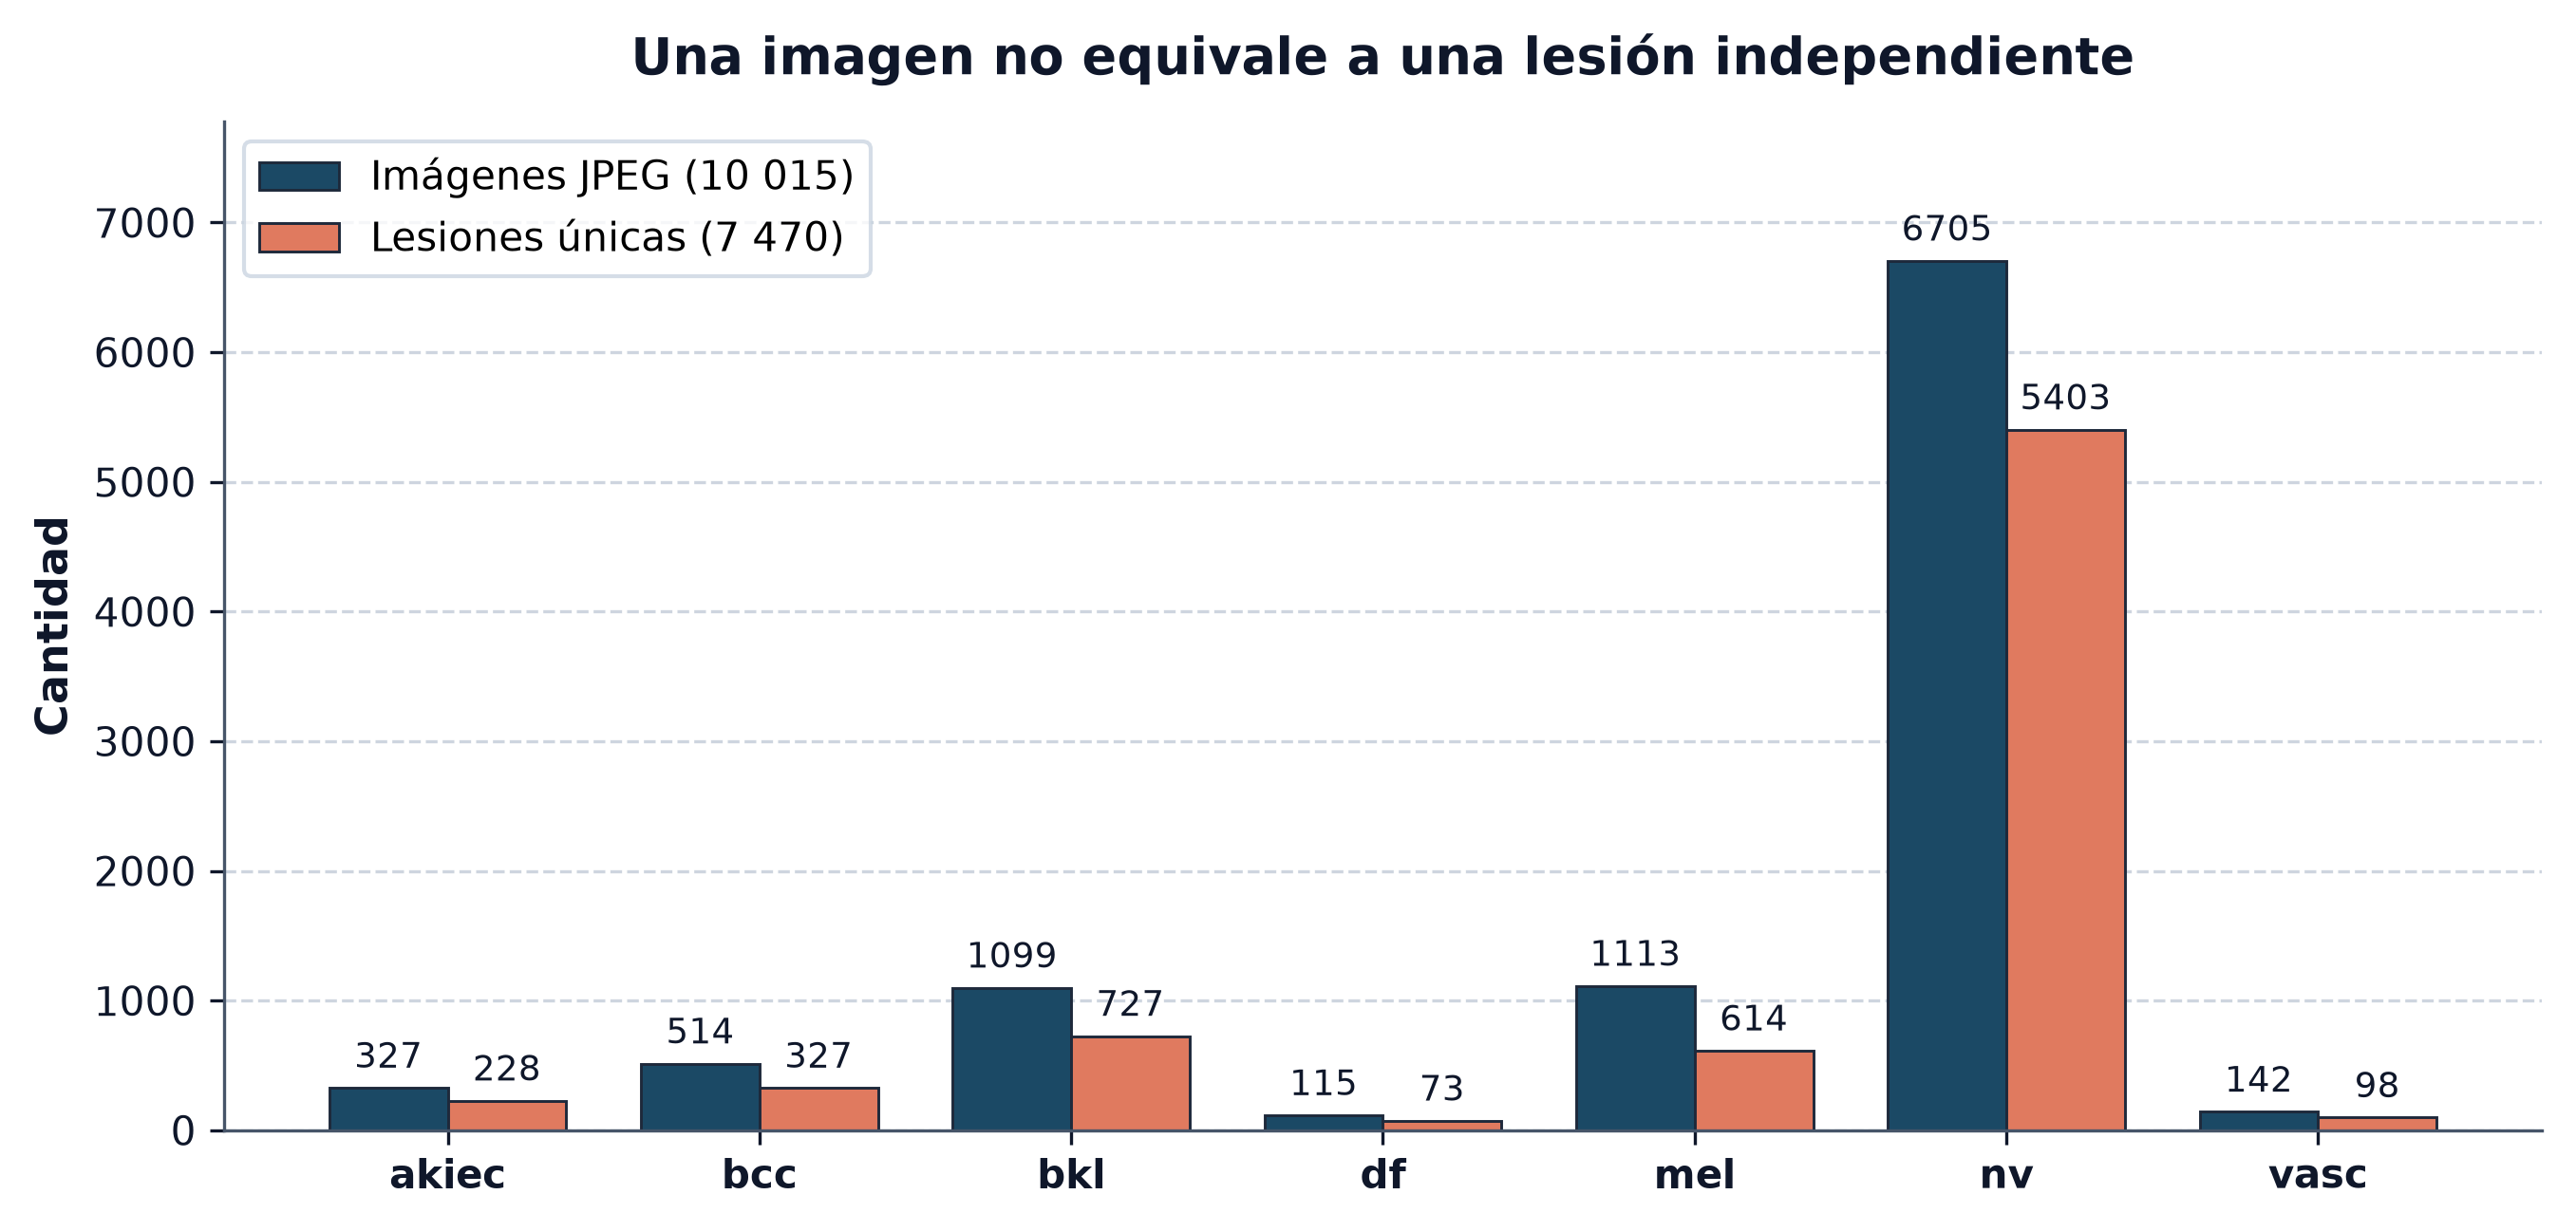
\includegraphics[width=\columnwidth]{02_lesiones.png}
\caption{Comparaci\'on real entre im\'agenes totales y lesiones \'unicas por clase, evidenciando dependencia muestral y desbalance.}
\label{fig:clases_split}
\end{figure}

\subsection{Preprocesamiento, Normalizaci\'on y Aumento de Datos}
El flujo general del sistema se ilustra en la Fig.~\ref{fig:pipeline}. Se descartan las matrices derivadas de $8\times8$ y $28\times28$ incluidas en el paquete de Kaggle porque degradan la textura dermatosc\'opica; en su lugar, se trabaja directamente con los JPEG originales convertidos a espacio RGB respetando orientaci\'on EXIF. Para evitar deformaci\'on anisotr\'opica de los bordes de la lesi\'on, cada imagen de $600\times450$ p\'ixeles se adapta a $224\times224$ mediante redimensionamiento isotr\'opico (\textit{letterbox} bilineal) y relleno sim\'etrico con el color de la media ImageNet.

Tras escalar intensidades al rango $[0,1]$, se aplica normalizaci\'on est\'andar por canal:
\begin{equation}
x'_c = \frac{x_c - \mu_c}{\sigma_c}, \quad c \in \{R, G, B\},
\end{equation}
empleando los par\'ametros de preentrenamiento ImageNet $\mu=(0.485,0.456,0.406)$ y $\sigma=(0.229,0.224,0.225)$ requeridos por las tres redes \cite{torchvisiondocs}. De forma complementaria, la exportaci\'on de la estructura organizada \texttt{data/processed/\{train,val,test\}} registr\'o las estad\'isticas emp\'iricas calculadas exclusivamente sobre los 7\,009 ejemplos de entrenamiento ($\mu_{\mathrm{train}}=[0.693823, 0.523161, 0.529890]$, $\sigma_{\mathrm{train}}=[0.170584, 0.136846, 0.162109]$) sin contaminar validaci\'on ni prueba.

El aumento de datos se restringe exclusivamente al subconjunto \texttt{train} e incluye volteo horizontal ($p=0.5$), volteo vertical ($p=0.5$), rotaci\'on aleatoria en $[-30^\circ, +30^\circ]$ y perturbaci\'on moderada de brillo y contraste en $[0.9, 1.1]$ (Fig.~\ref{fig:prep}). Cada transformaci\'on aleatoria deriva su semilla determinista de la tupla $(\text{semilla}, \text{\'epoca}, \texttt{image\_id})$, evitando que la variaci\'on del estado RNG interno entre modelos altere la secuencia de aumentos recibida.

\begin{figure*}[t]
\centering
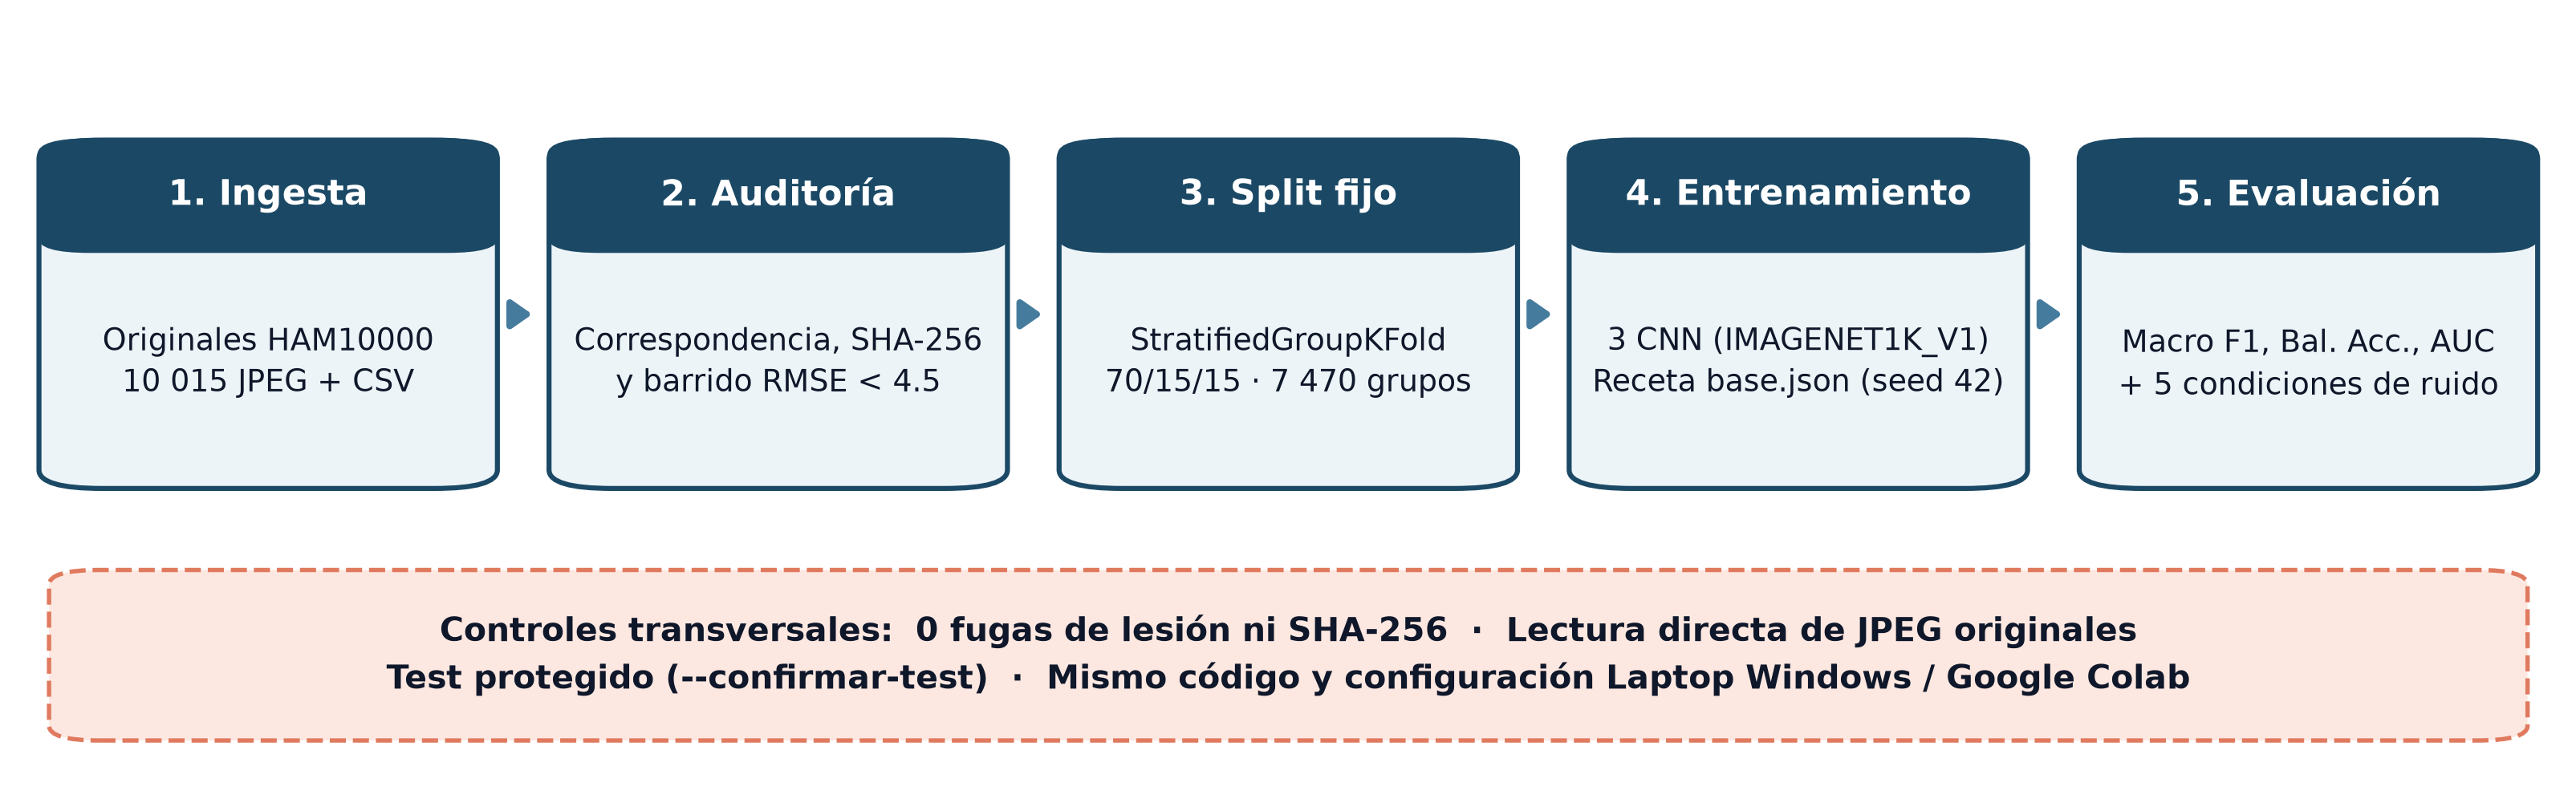
\includegraphics[width=0.86\textwidth]{10_pipeline.png}
\caption{Flujo metodol\'ogico unificado del estudio: preservaci\'on de originales, auditor\'ia, split fijo, entrenamiento y evaluaci\'on.}
\label{fig:pipeline}
\end{figure*}

\begin{figure}[t]
\centering
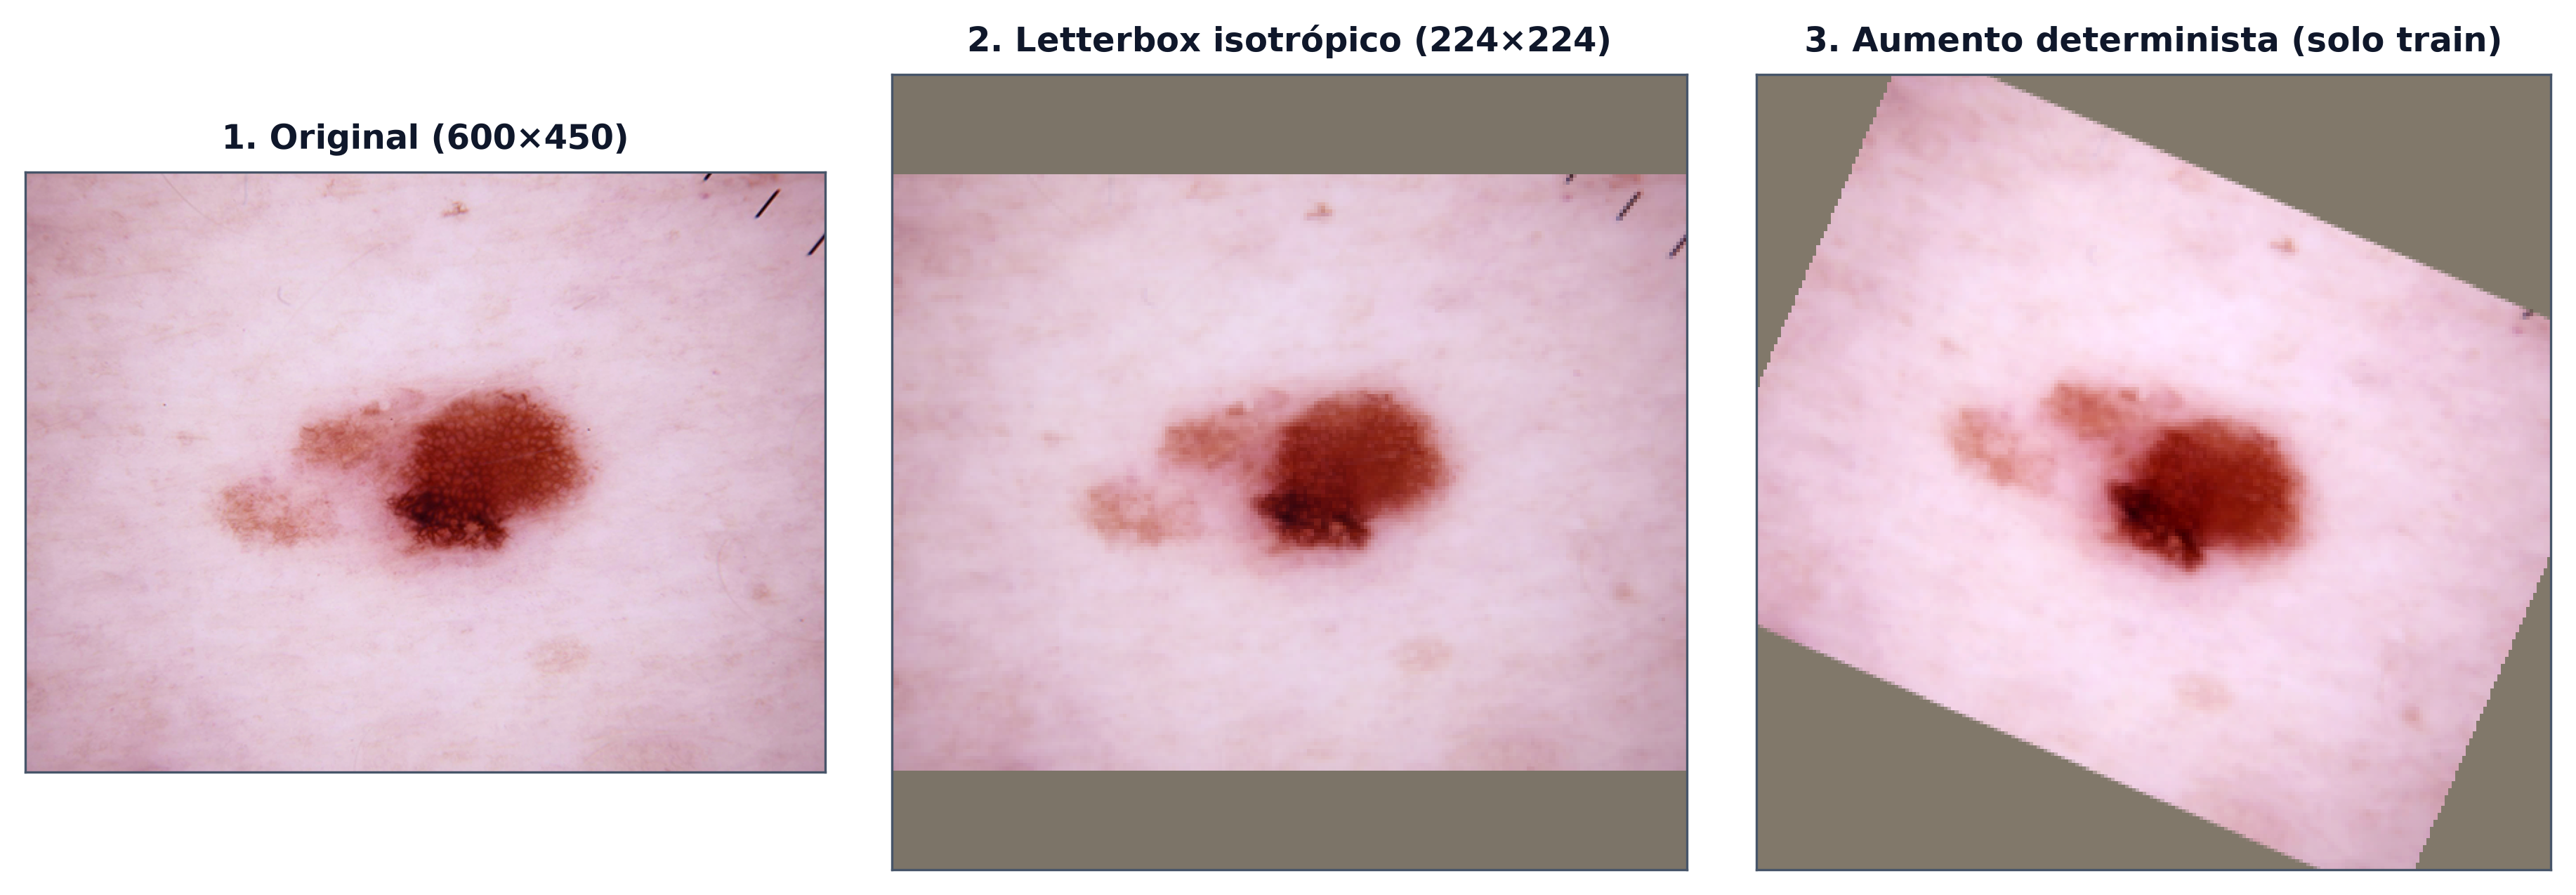
\includegraphics[width=\columnwidth]{08_preprocesamiento.png}
\caption{Ejemplo real de entrenamiento: original $600\times450$, adaptaci\'on isotr\'opica $224\times224$ y aumento en l\'inea (desnormalizado para visualizaci\'on).}
\label{fig:prep}
\end{figure}

\subsection{Arquitecturas CNN Comparadas}
Se seleccionan tres arquitecturas de aprendizaje profundo de complejidad y dise\~no distintos dentro de \texttt{torchvision}, reemplazando su capa clasificadora final por una proyecci\'on lineal a siete salidas \cite{torchvisiondocs} (Fig.~\ref{fig:arqs} y Cuadro~\ref{tab:modelos}):

\begin{enumerate}
\item \textbf{ResNet-18:} modelo residual de referencia con bloques convolucionales $3\times3$ e identidad aditiva $y = \mathcal{F}(x; \{W_i\}) + x$ (o proyecci\'on lineal cuando cambian dimensiones) \cite{he2016}. Aporta 11\,180\,103 par\'ametros entrenables tras adaptar la capa \texttt{fc} de 512 a 7 salidas.
\item \textbf{EfficientNet-B0:} arquitectura dise\~nada mediante b\'usqueda neuronal y escalado compuesto de profundidad ($d=\alpha^\phi$), ancho ($w=\beta^\phi$) y resoluci\'on ($r=\gamma^\phi$) con restricci\'on $\alpha\cdot\beta^2\cdot\gamma^2\approx 2$ \cite{tan2019}. Integra bloques invertidos \textit{MBConv} y atenci\'on de canales SE, sumando 4\,016\,515 par\'ametros para siete clases.
\item \textbf{MobileNetV3-Small:} red compacta optimizada para baja latencia mediante convoluciones separables en profundidad, cuellos de botella invertidos con expansi\'on ligera, m\'odulos SE y activaciones \textit{hard-swish} y \textit{ReLU} \cite{howard2019}. Su variante adaptada consta de 1\,525\,031 par\'ametros.
\end{enumerate}

\begin{figure*}[t]
\centering
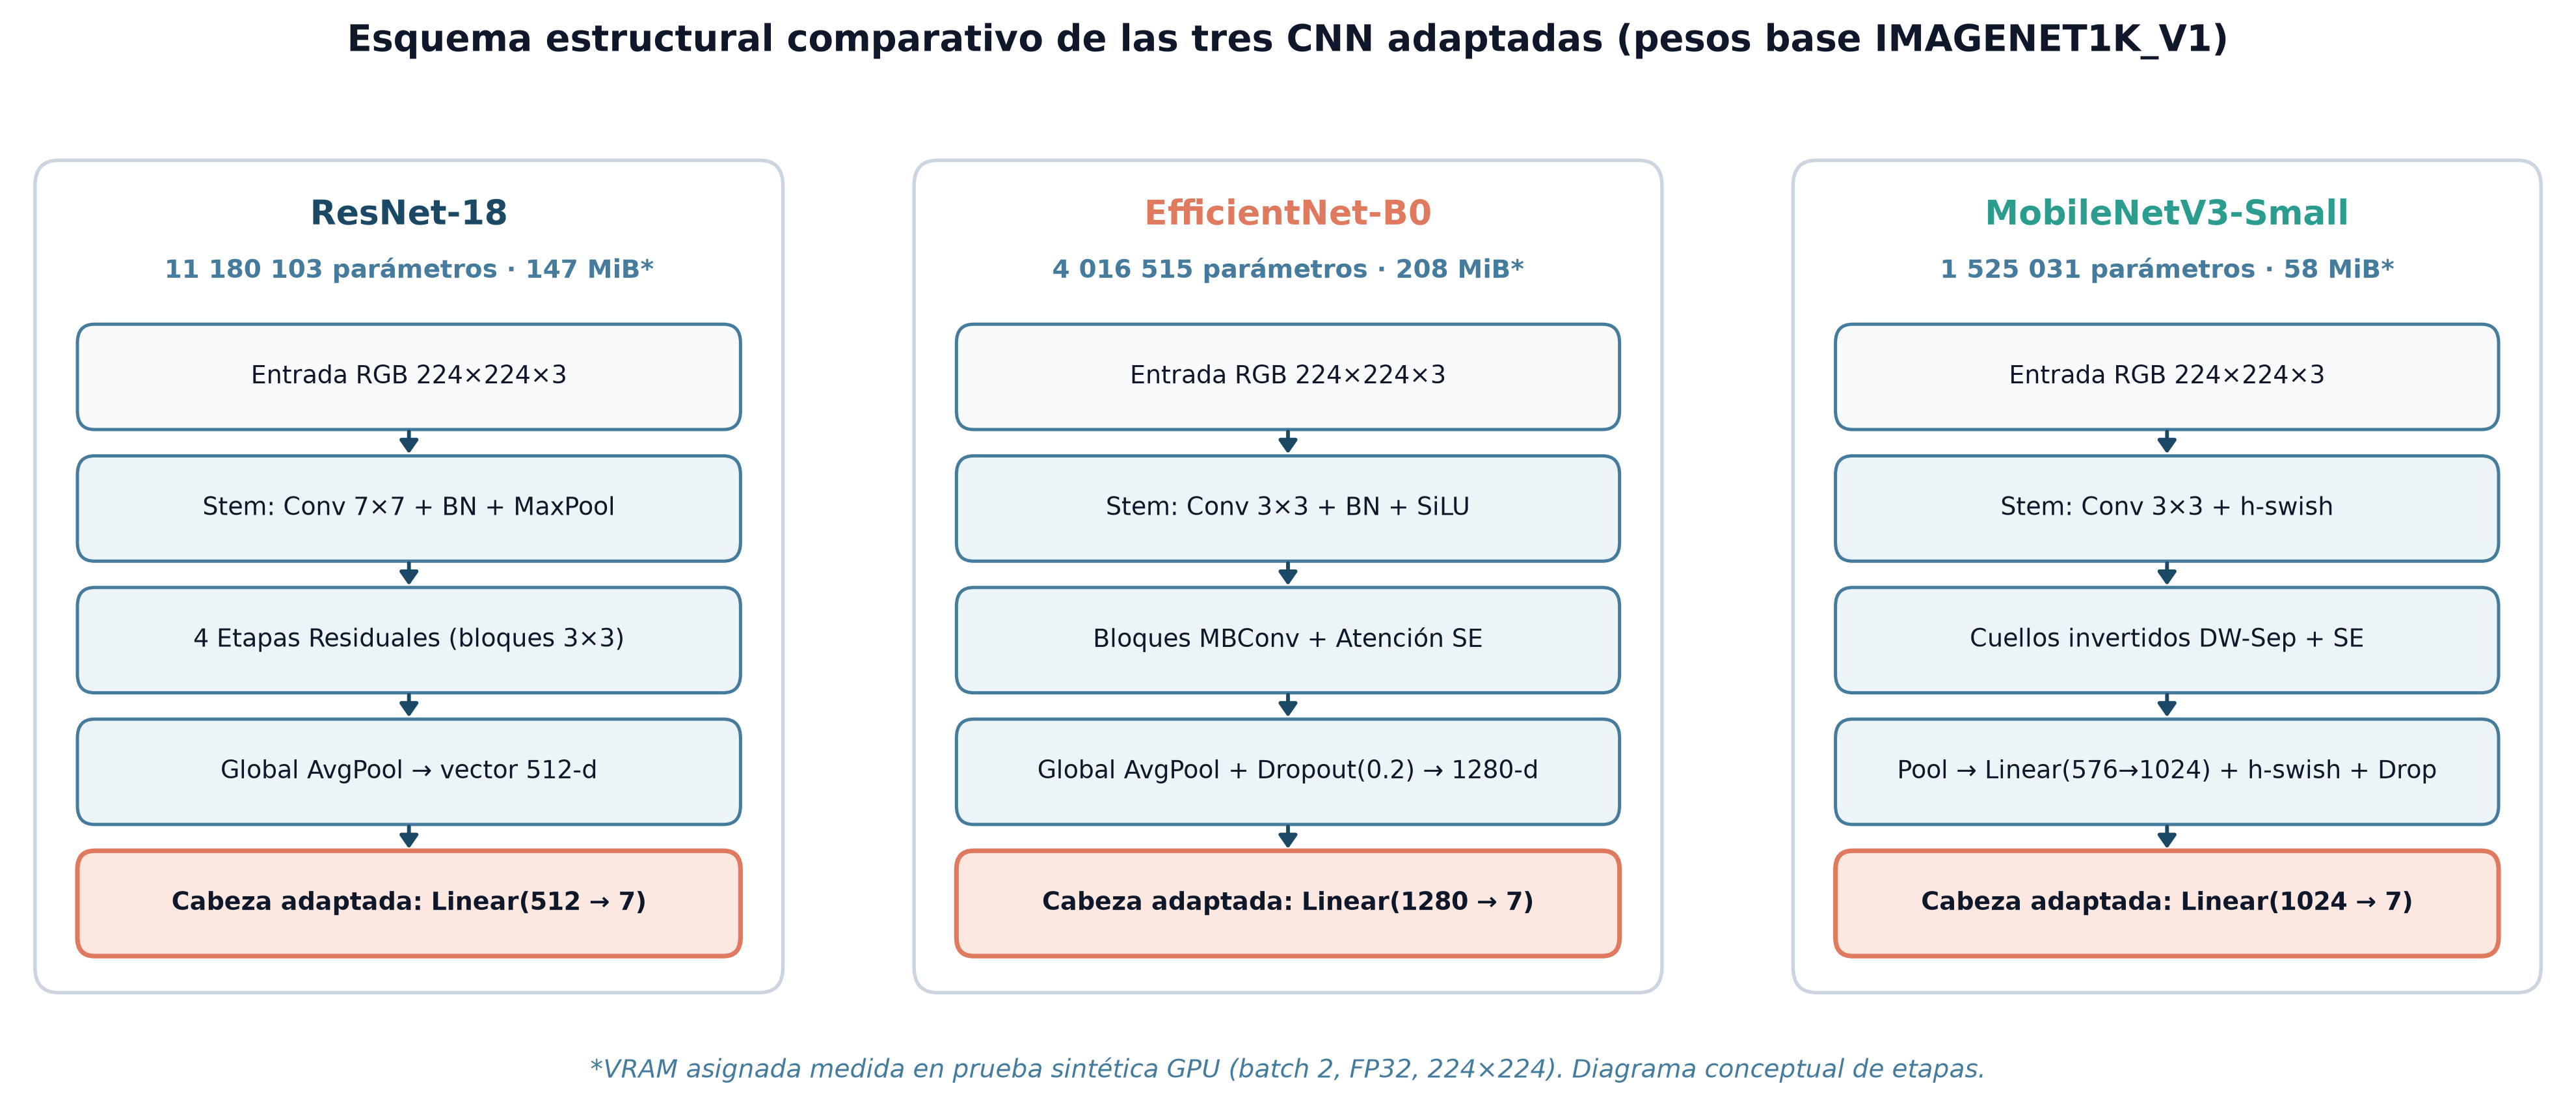
\includegraphics[width=0.86\textwidth]{11_arquitecturas.png}
\caption{Esquema conceptual comparativo de los bloques principales de ResNet-18, EfficientNet-B0 y MobileNetV3-Small adaptados a siete clases.}
\label{fig:arqs}
\end{figure*}

\begin{figure}[t]
\centering
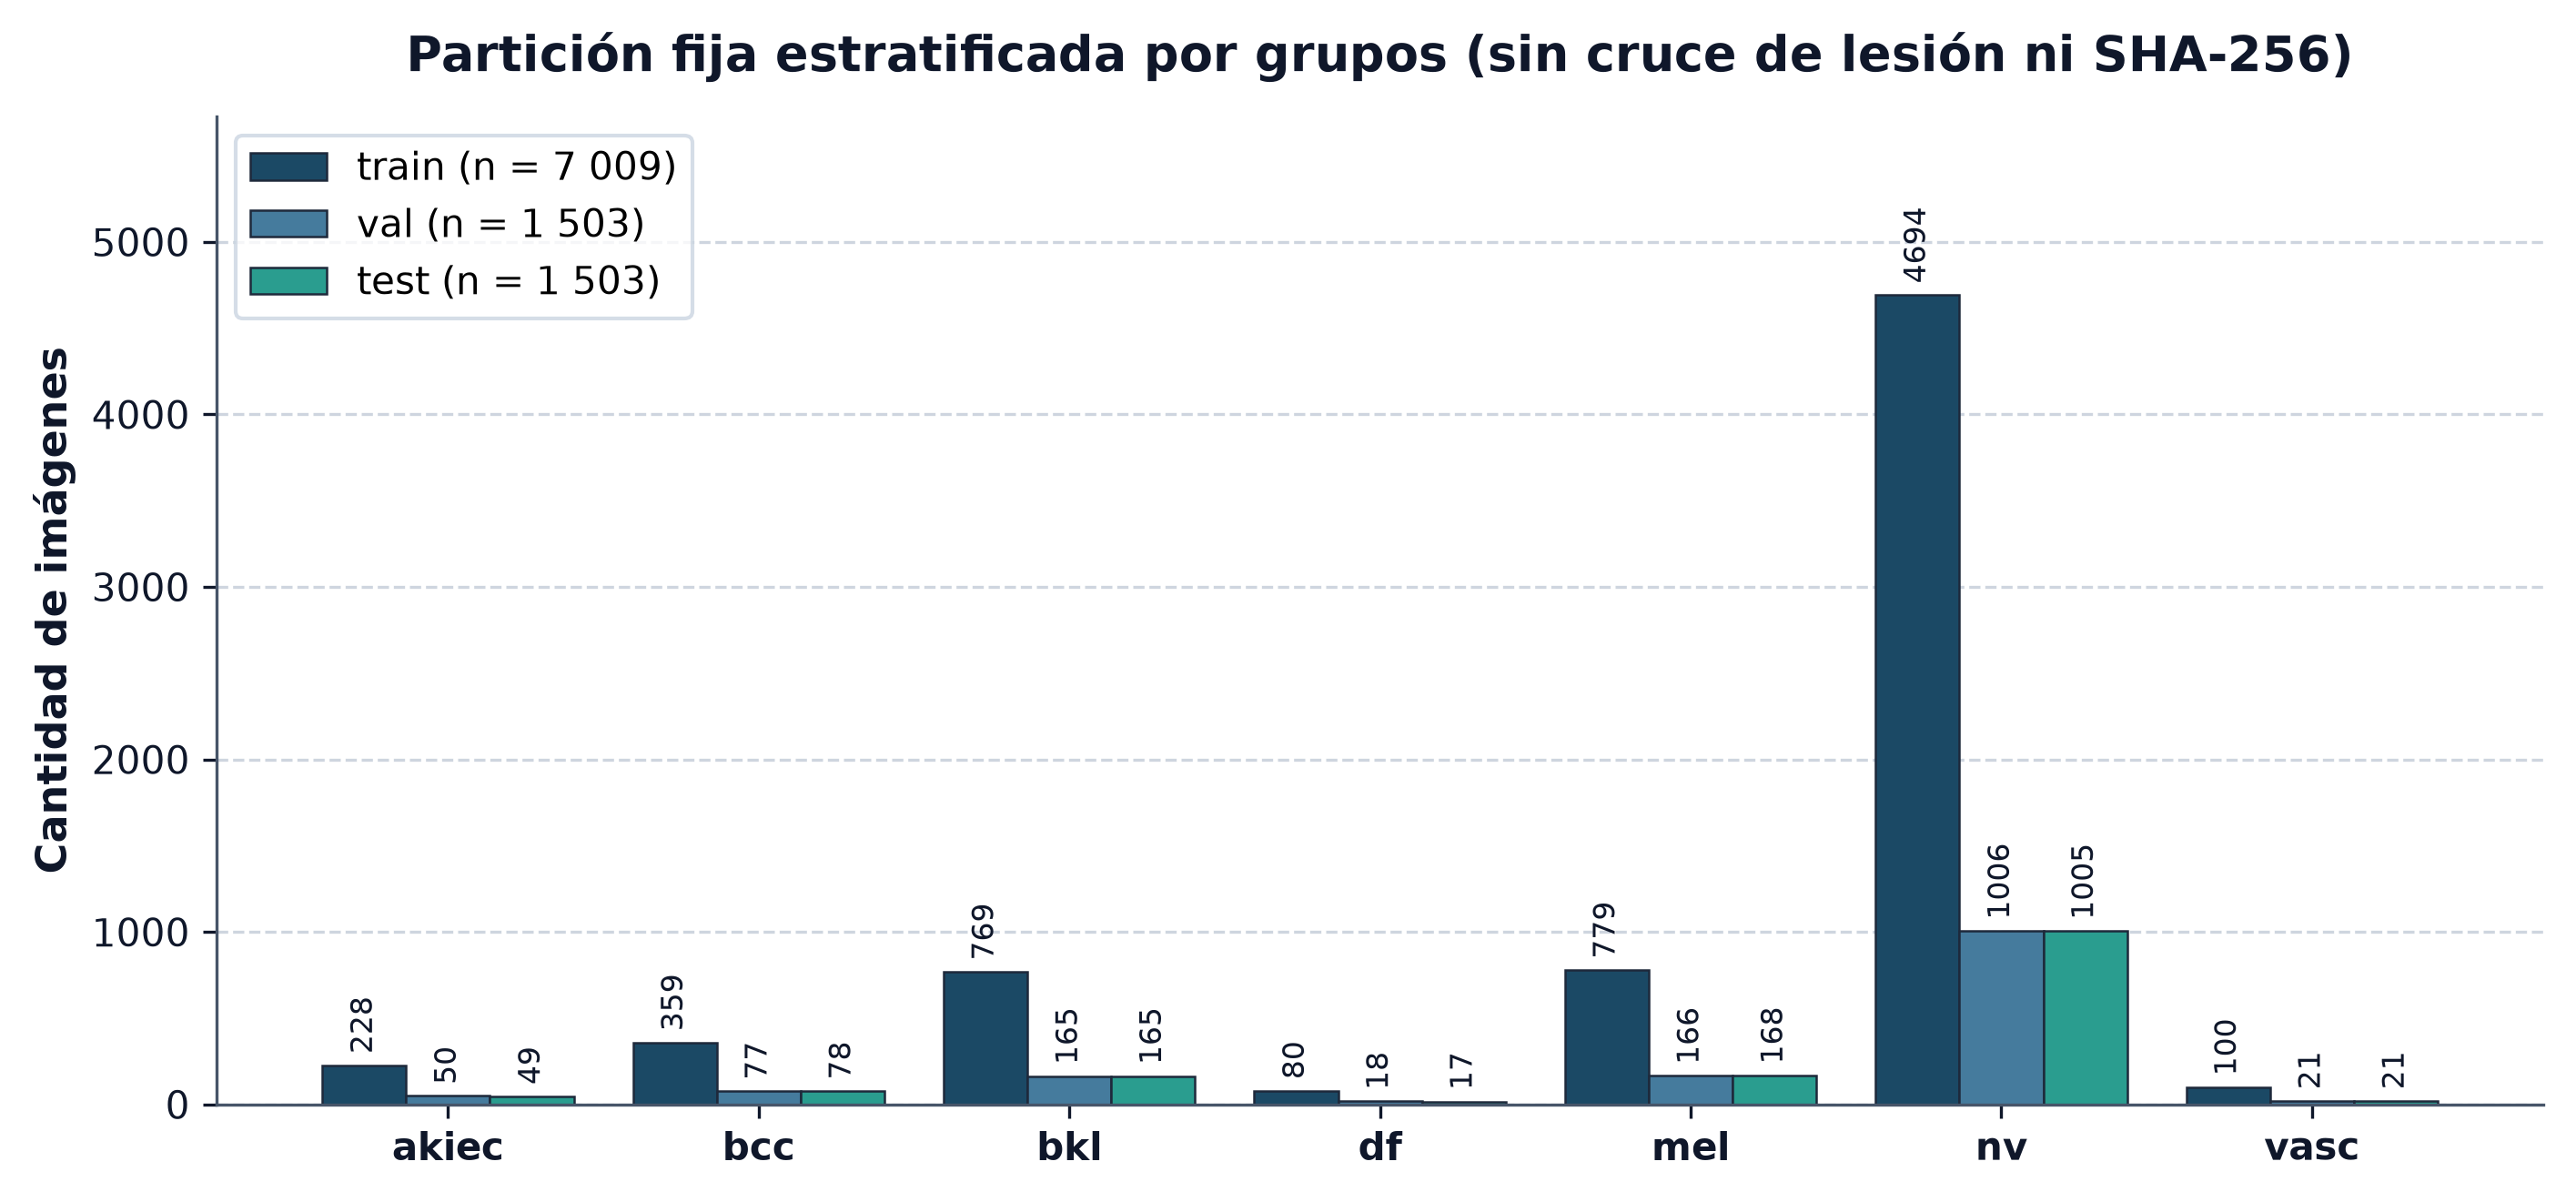
\includegraphics[width=\columnwidth]{04_split.png}
\caption{Conteos reales de la partici\'on estratificada por grupos (\texttt{train}: 7\,009, \texttt{val}: 1\,503, \texttt{test}: 1\,503) con las siete clases presentes en los tres conjuntos.}
\label{fig:split_bars}
\end{figure}

\begin{table}[t]
\centering\scriptsize
\setlength{\tabcolsep}{4pt}
\caption{Especificaci\'on de las tres CNN adaptadas a HAM10000.}
\label{tab:modelos}
\begin{tabular}{lllr}\toprule
Modelo & Mecanismo & Pesos base & Par\'ametros \\ \midrule
ResNet-18 & Residuales & \texttt{IMAGENET1K\_V1} & 11\,180\,103 \\
EfficientNet-B0 & MBConv + SE & \texttt{IMAGENET1K\_V1} & 4\,016\,515 \\
MobileNetV3-Small & Sep. + SE & \texttt{IMAGENET1K\_V1} & 1\,525\,031 \\
\bottomrule\end{tabular}
\end{table}

\subsection{Entrenamiento, Control Experimental y Entorno H\'ibrido}
Todos los modelos comparten exactamente la configuraci\'on declarativa de \texttt{configs/base.json} (Cuadro~\ref{tab:config}). Para compensar el desbalance sin recurrir a sobremuestreo sint\'etico en disco, se utiliza entrop\'ia cruzada ponderada sobre \texttt{train} mediante \texttt{CrossEntropyLoss(weight=..., reduction='mean')} en PyTorch:
\begin{equation}
\mathcal{L}_{\mathrm{CE}} = -\frac{\sum_{i=1}^{B} w_{y_i}\log p_{i,y_i}}{\sum_{i=1}^{B} w_{y_i}}, \qquad w_c = \frac{N_{\mathrm{train}}}{K\,n_c},
\end{equation}
donde $K=7$, $N_{\mathrm{train}}=7\,009$, $n_c$ corresponde exclusivamente a la frecuencia en entrenamiento (valores en Cuadro~\ref{tab:split}) y el denominador normaliza por la suma de los pesos de las etiquetas del lote (y no por $B$), coincidiendo exactamente con la implementaci\'on en PyTorch. La implementaci\'on se apoya en PyTorch y scikit-learn \cite{pytorch2019,sklearn2011}, verificando compatibilidad del controlador NVIDIA~621.01 sobre la laptop Acer Nitro AN515-45 \cite{nvidiadriver,acerdrivers}.

\begin{table}[t]
\centering\scriptsize
\setlength{\tabcolsep}{4pt}
\caption{Protocolo de entrenamiento e infraestructura ejecutada.}
\label{tab:config}
\begin{tabular}{ll}\toprule
Par\'ametro / Recurso & Configuraci\'on verificada \\ \midrule
Resoluci\'on / Lote & RGB $224\times224$ / Batch 8 (\texttt{workers}=4) \\
\'Epocas m\'aximas & 20 (2 cabeza + hasta 18 ajuste) \\
Optimizador & AdamW (weight decay $10^{-4}$) \\
Tasas (cabeza / base) & $10^{-4}$ / $10^{-5}$ (decaimiento coseno) \\
Criterio / Parada & Macro F1 en \texttt{val} / paciencia 5 \\
Semilla / Precisi\'on & 42 / FP32 (recorte gradiente $L_2=1.0$) \\
Entorno ejecutado & Acer Nitro AN515-45, GTX 1650 (4~GiB) \\
Software GPU & Driver 621.01, PyTorch 2.11.0+cu128 \\
Portabilidad prevista & Colab + Drive; nube no acreditada \cite{colabfaq} \\
\bottomrule\end{tabular}
\end{table}

Durante las dos primeras \'epocas se congelan los pesos del extractor y se fijan las capas de \textit{BatchNorm} en modo \texttt{eval()} para preservar estad\'isticas preentrenadas mientras converge la cabeza. Posteriormente se descongela la red completa con decaimiento coseno y tasas diferenciadas. Cada \'epoca completa guarda \texttt{last.pt} de forma at\'omica y actualiza \texttt{best.pt} si mejora validaci\'on, incluyendo optimizador y generadores para reanudar desde la \'ultima \'epoca completa. Tras un piloto puntual de sesi\'on con workers 0 y 4 en Windows (sin reporte independiente persistido), los entrenamientos y mediciones finales se ejecutaron con \texttt{num\_workers=4} sobre la misma GTX~1650.

El cuaderno integrado local/Colab comparte paquete, t\'itulo, configuraci\'on y split; no importa Drive fuera del backend alojado ni cambia workers autom\'aticamente. Inicia con entrenamiento y evaluaci\'on desactivados, distingue referencias locales de ejecuciones nuevas y detecta evaluaciones incompletas. Se verificaron esquema, sintaxis y ejecuci\'on local de inspecci\'on; la rama de nube se simul\'o, \textbf{sin ejecuci\'on real acreditada en Colab}. La reanudaci\'on conserva el protocolo y no garantiza identidad bit a bit entre dispositivos.

\section{Protocolo de Evaluaci\'on y Robustez}

\subsection{Evaluaci\'on Multim\'etrica}
Siguiendo el principio de no restringirse a \textit{Accuracy}, se calculan por clase la precisi\'on ($\mathrm{Precision}_c = TP_c / (TP_c+FP_c)$), la sensibilidad o exhaustividad ($\mathrm{Recall}_c = TP_c / (TP_c+FN_c)$) y el puntaje $F1_c$. La m\'etrica primaria de selecci\'on y comparaci\'on es el Macro~F1, complementado con exactitud balanceada y sensibilidad espec\'ifica de melanoma:
\begin{equation}
\mathrm{Macro\text{-}F1} = \frac{1}{7}\sum_{c=1}^{7} F1_c, \qquad
\mathrm{Bal.\ Acc.} = \frac{1}{7}\sum_{c=1}^{7} \mathrm{Recall}_c.
\end{equation}
Se calcula adem\'as el \'area bajo la curva ROC multiclase uno contra el resto ($\mathrm{AUC}_{\mathrm{OVR}}$), consolidando curvas ROC comparativas, barras de desempe\~no/eficiencia, matrices de confusi\'on y predicciones por muestra. Dado que la tarea es clasificaci\'on de etiqueta \'unica sin m\'ascaras ni cajas, IoU, Dice o mAP no aplican.

\subsection{An\'alisis de Sensibilidad, Mitigaci\'on y Eficiencia}
Una vez congelados los mejores checkpoints mediante \texttt{val}, se eval\'uan cinco condiciones deterministas sobre \texttt{test} (Fig.~\ref{fig:robustez}): referencia limpia (\texttt{clean}), ruido gaussiano aditivo con $\sigma \in \{0.02, 0.05\}$ sobre intensidades $[0,1]$ y desenfoque gaussiano con radios $r \in \{1, 2\}$ p\'ixeles. La semilla del ruido depende del identificador de imagen, garantizando perturbaciones id\'enticas para las tres CNN. La ca\'ida de robustez se mide con $\Delta \mathrm{Macro\text{-}F1} = \mathrm{Macro\text{-}F1}_{\mathrm{clean}} - \mathrm{Macro\text{-}F1}_{\mathrm{perturbado}}$. Sobre la condici\'on severa \texttt{noise\_005}, se aplica mitigaci\'on espacial previa a la normalizaci\'on mediante filtro de mediana $3\times 3$ (\texttt{+median\_3}) o gaussiano $r=1$ (\texttt{+gaussian\_1}). La eficiencia registra par\'ametros, VRAM, tiempo por \'epoca y mediana/P95 de latencia \texttt{forward()} (batch 1, FP32, 10 calentamientos y 50 mediciones sincronizadas), sin E/S, preprocesamiento ni filtrado CPU. La suite revisada aprob\'o 22 pruebas de pipeline/cuaderno y 4 de descarga, incluidas reanudaci\'on entre \'epocas sint\'eticas, evaluaci\'on CPU de checkpoint CUDA y protecci\'on de artefactos.

\begin{figure*}[t]
\centering
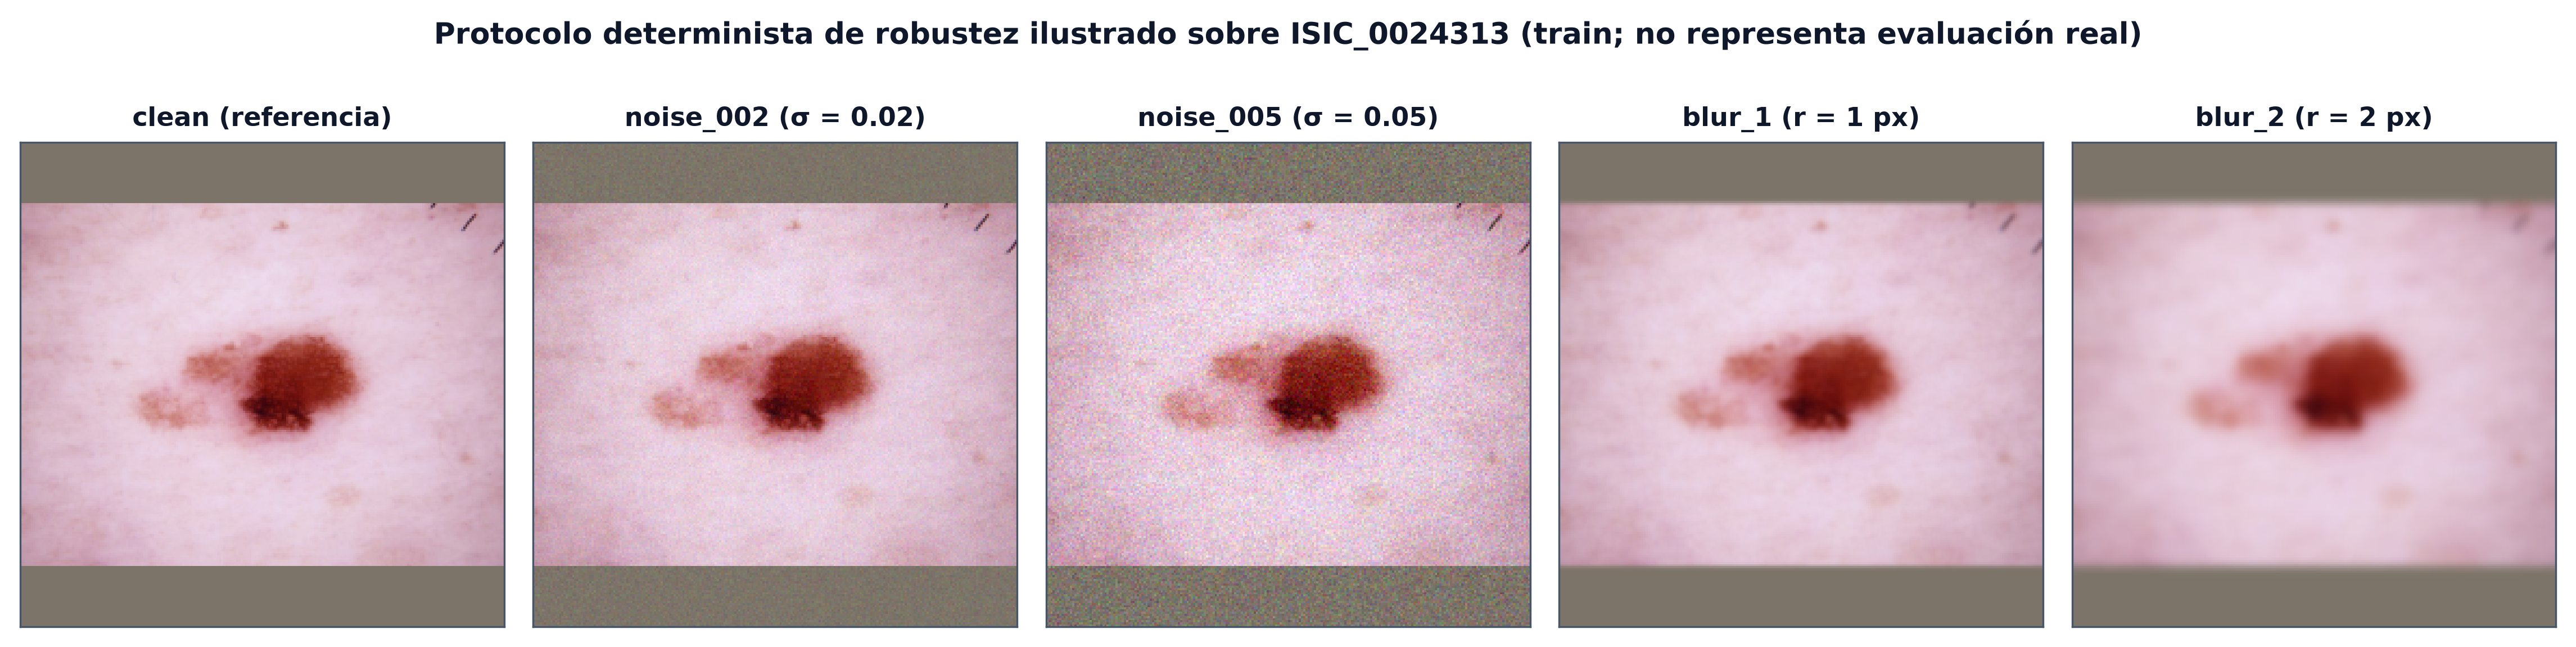
\includegraphics[width=0.84\textwidth]{09_robustez.png}
\caption{Condiciones deterministas de robustez aplicadas a \texttt{test} (ilustrado sobre una muestra de entrenamiento).}
\label{fig:robustez}
\end{figure*}

\section{Resultados}

\subsection{Entrenamiento y Convergencia en GPU Local}
Bajo la configuraci\'on congelada en GTX~1650 (FP32, \texttt{batch=8}, \texttt{num\_workers=4}, \texttt{seed=42}), \textbf{ResNet-18} activ\'o parada temprana en la \'epoca~16 tras alcanzar su mejor punto en la \'epoca~11 con Macro~F1 en \texttt{val} de $0.6927$, completando $2\,040.7$~s totales ($127.5$~s/\'epoca) y $434.2$~MiB de VRAM pico. \textbf{EfficientNet-B0} complet\'o las 20~\'epocas con su mejor registro en la \'epoca~19 (Macro~F1 en \texttt{val} de $0.7059$), requiriendo $3\,771.2$~s ($188.6$~s/\'epoca) y $805.7$~MiB de VRAM. \textbf{MobileNetV3-Small} se detuvo en la \'epoca~19 (mejor \'epoca~14, Macro~F1 en \texttt{val} de $0.6213$) en $2\,970.4$~s ($156.3$~s/\'epoca) y apenas $211.8$~MiB de VRAM.

\subsection{Desempe\~no en Test Limpio y Eficiencia Computacional}
El Cuadro~\ref{tab:res} y la Fig.~\ref{fig:comp_metricas} sintetizan la evaluaci\'on sobre las $1\,503$ im\'agenes limpias de \texttt{test}. \textbf{ResNet-18} ofrece el mejor compromiso observado en este protocolo y GPU: lidera en Accuracy ($0.8031$), Macro~F1 ($0.6786$), exactitud balanceada ($0.7174$) y AUC~OVR ($0.9596$), con Macro~Prec.\ de $0.6591$, a la vez que registra la menor latencia \texttt{forward()} (\texttt{batch=1}) en limpio ($7.22$~ms de mediana; $\mathrm{P95}=8.09$~ms) y el entrenamiento m\'as r\'apido ($127.5$~s/\'epoca). \textbf{EfficientNet-B0} obtiene la mayor Macro~Prec.\ ($0.6741$) y la mayor sensibilidad limpia en melanoma ($0.6607$ frente a $0.6012$ de ResNet-18), en l\'inea con su mayor AUC espec\'ifico de melanoma (Fig.~\ref{fig:roc_comp}: $0.911$ vs.\ $0.895$ y $0.859$), y registra un Macro~F1 muy cercano ($0.6778$). No obstante, la diferencia puntual de Macro~F1 ($\Delta=0.00084$) no demuestra superioridad estad\'istica ni equivalencia formal: un bootstrap pareado sobre los $1\,118$ grupos independientes de \texttt{test} arroja un IC95\% de $[-0.0429, +0.0464]$. Adicionalmente, su costo computacional en GPU es mayor ($805.7$~MiB de VRAM y $24.60$~ms de latencia mediana \texttt{forward()}, $\mathrm{P95}=25.97$~ms). Por su parte, \textbf{MobileNetV3-Small} reduce la memoria pico a $211.8$~MiB con Macro~Prec.\ de $0.6474$, pero desciende a $0.5700$ en Macro~F1, $0.5604$ en exactitud balanceada y $0.4167$ en Recall de melanoma, con $22.40$~ms en limpio ($\mathrm{P95}=23.97$~ms). A lo largo de las siete evaluaciones sobre \texttt{test}, la latencia mediana \texttt{forward()} (\texttt{batch=1}, sin E/S ni filtrado en CPU) mostr\'o variabilidad entre corridas de $6.86\text{--}9.46$~ms (ResNet-18), $15.26\text{--}22.40$~ms (MobileNetV3-Small) y $22.49\text{--}34.82$~ms (EfficientNet-B0).

\begin{table*}[t]
\centering\scriptsize
\setlength{\tabcolsep}{3.5pt}
\caption{Desempe\~no en conjunto \texttt{test} limpio ($n=1\,503$) y eficiencia computacional en GPU NVIDIA GTX~1650 (\texttt{forward()} \texttt{batch=1}).}
\label{tab:res}
\begin{tabular}{lccccccccc}\toprule
Arquitectura & Acc. & Macro Prec. & Macro F1 & Bal.\ Acc. & Recall \texttt{mel} & AUC OVR & s/\'epoca & Lat.\ med.\ (P95) ms & VRAM (MiB) \\ \midrule
ResNet-18 & \textbf{0.8031} & 0.6591 & \textbf{0.6786} & \textbf{0.7174} & 0.6012 & \textbf{0.9596} & \textbf{127.5} & \textbf{7.22} (8.09) & 434.2 \\
EfficientNet-B0 & 0.8004 & \textbf{0.6741} & 0.6778 & 0.7025 & \textbf{0.6607} & 0.9587 & 188.6 & 24.60 (25.97) & 805.7 \\
MobileNetV3-Small & 0.7625 & 0.6474 & 0.5700 & 0.5604 & 0.4167 & 0.9407 & 156.3 & 22.40 (23.97) & \textbf{211.8} \\
\bottomrule\end{tabular}
\end{table*}

\begin{figure*}[b]
\centering
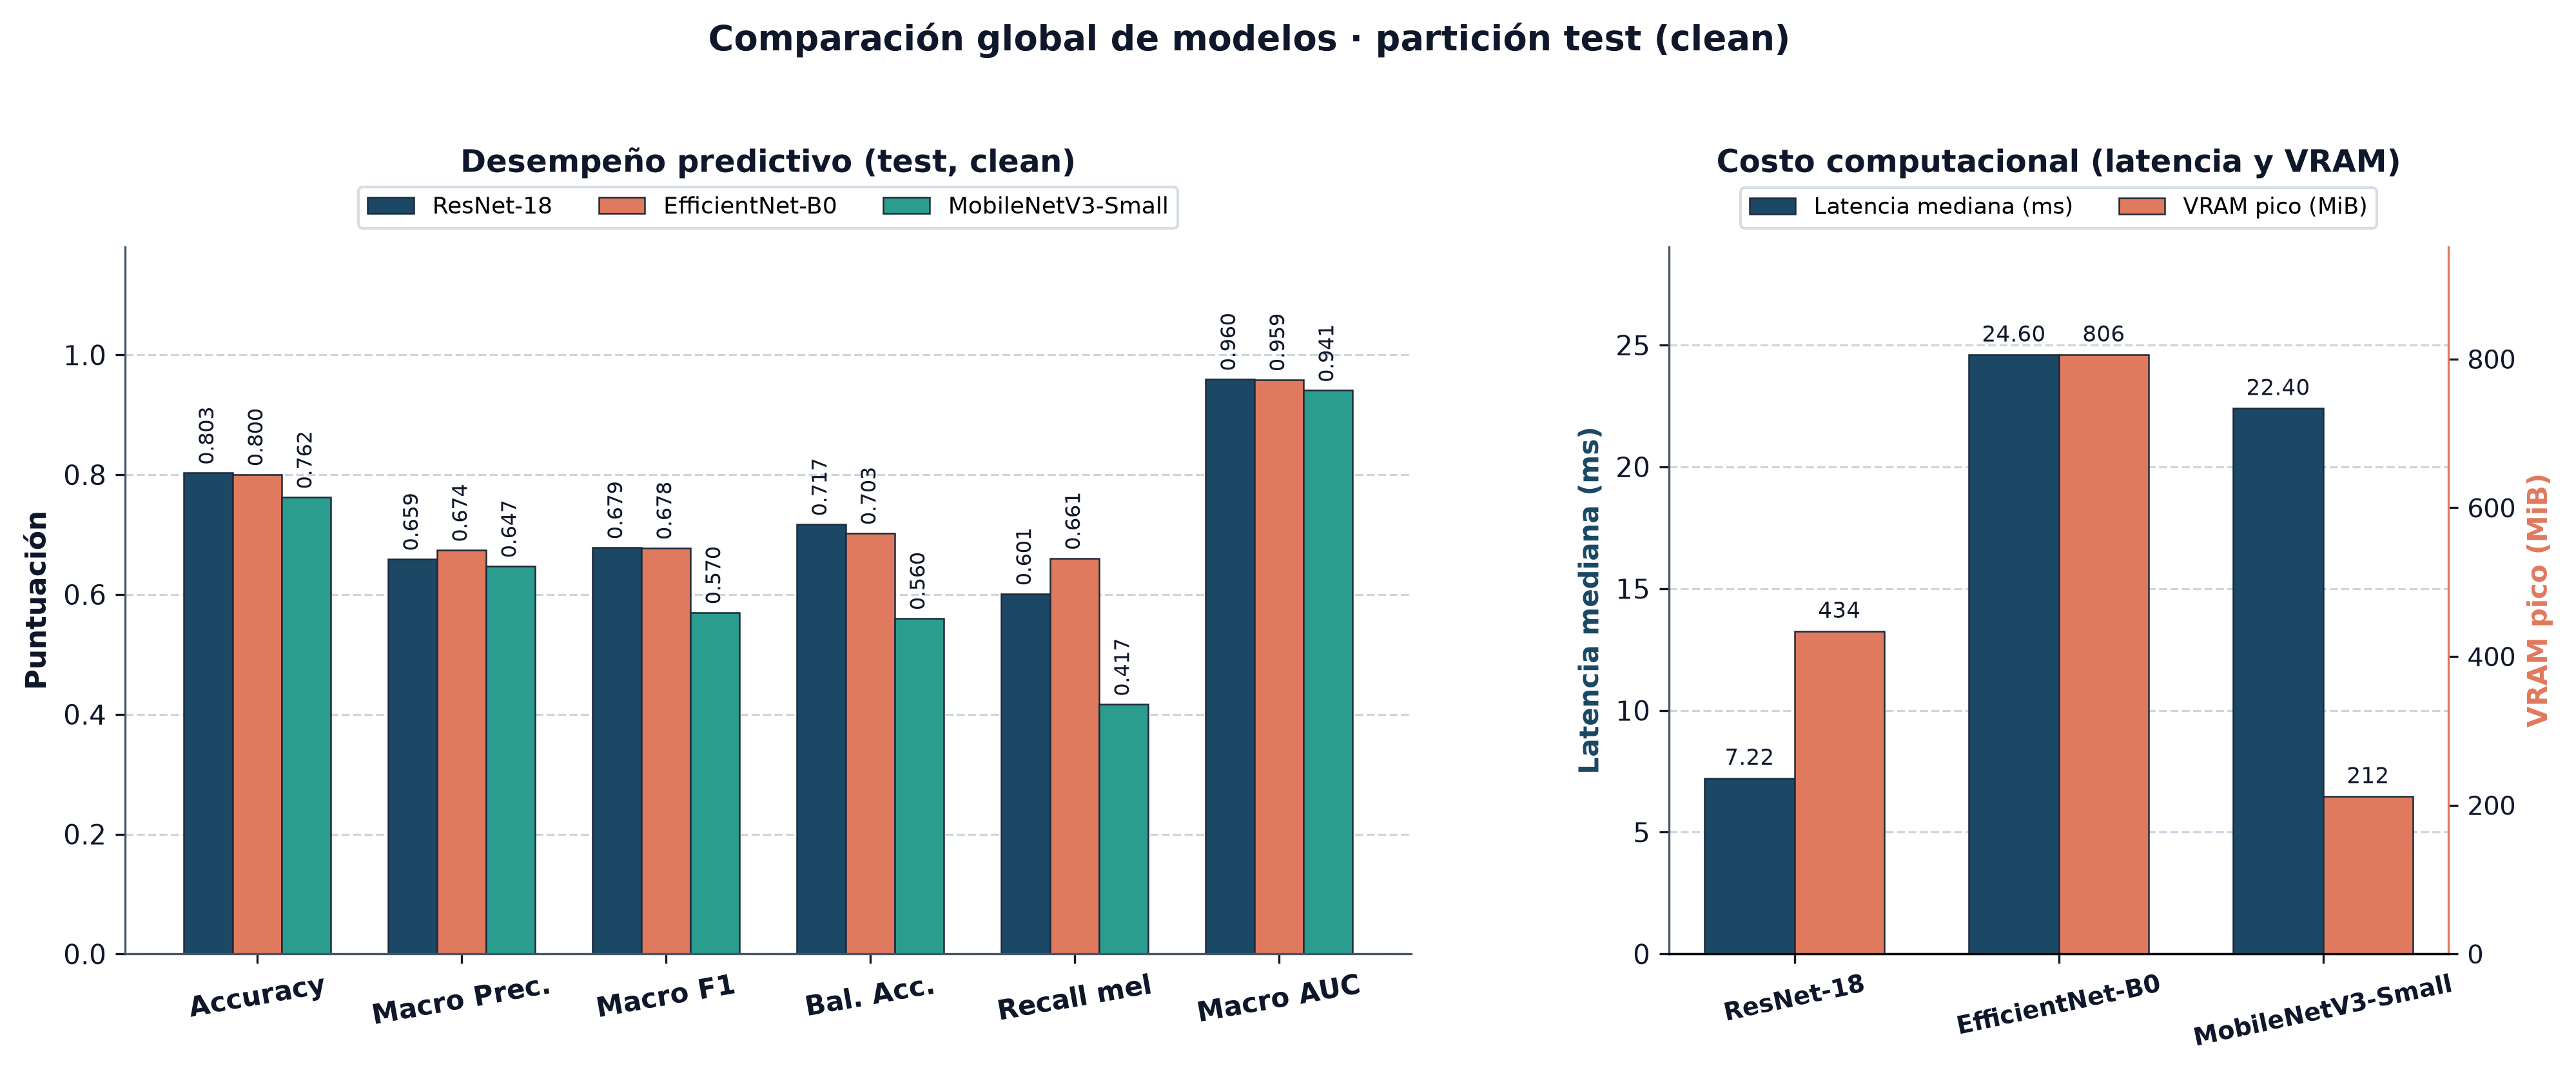
\includegraphics[width=0.76\textwidth]{comparacion_metricas.png}
\caption{Comparaci\'on en \texttt{test} limpio ($n=1\,503$): m\'etricas predictivas (izquierda) y costo computacional \texttt{forward()} con \texttt{batch=1} en GTX~1650 (derecha). ResNet-18 combina m\'aximo Macro~F1 observado ($0.6786$) y m\'inima latencia ($7.22$~ms), mientras EfficientNet-B0 maximiza Macro~Prec.\ ($0.6741$) y Recall \texttt{mel} ($0.6607$) a costa de mayor VRAM ($805.7$~MiB).}
\label{fig:comp_metricas}
\end{figure*}

\begin{figure*}[t]
\centering
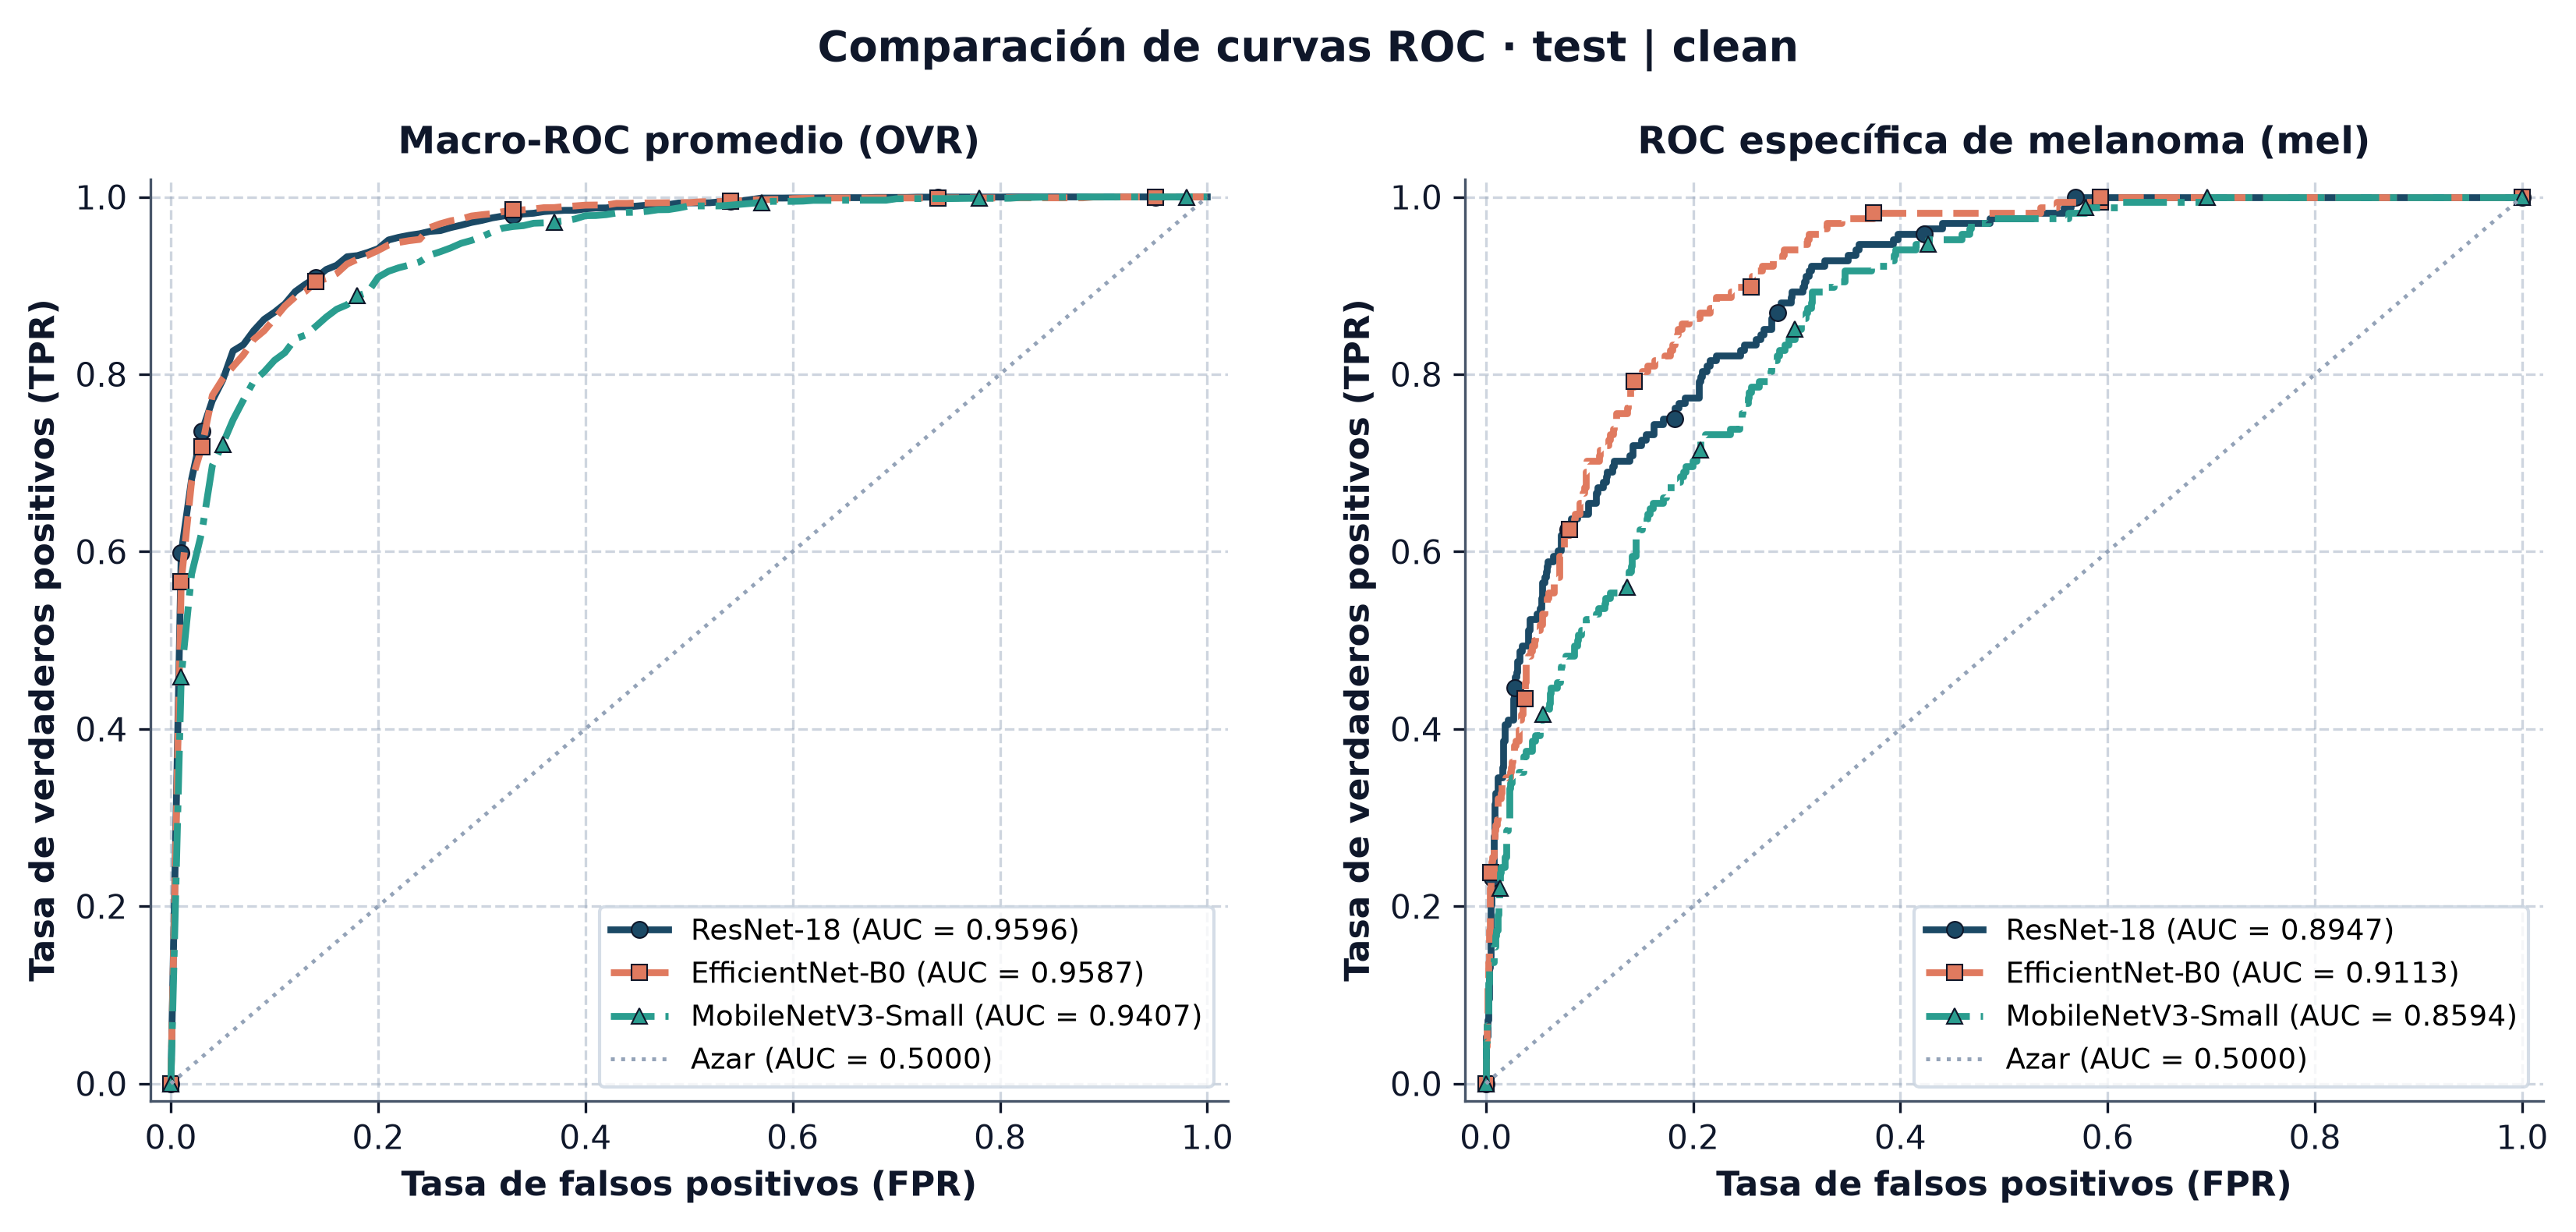
\includegraphics[width=0.76\textwidth]{roc_comparativa_test_clean.png}
\caption{Curvas ROC comparativas en \texttt{test} limpio: Macro-ROC promedio OVR (izquierda; AUC exacto de $0.9596$, $0.9587$ y $0.9407$) y ROC espec\'ifica de melanoma (derecha), donde EfficientNet-B0 alcanza $\mathrm{AUC}=0.911$ frente a $0.895$ de ResNet-18 y $0.859$ de MobileNetV3-Small.}
\label{fig:roc_comp}
\end{figure*}

\subsection{Robustez ante Perturbaciones y Mitigaci\'on Espacial}
El Cuadro~\ref{tab:rob} y la Fig.~\ref{fig:comp_robustez} detallan la sensibilidad ante ruido aditivo y desenfoque. El ruido gaussiano degrada el Macro~F1 de forma m\'as pronunciada que el desenfoque: en \texttt{noise\_005}, \textbf{EfficientNet-B0} sufre un colapso severo hasta $0.1201$ ($\Delta\mathrm{F1}=+0.5577$, Recall \texttt{mel} $0.0000$), \textbf{ResNet-18} desciende a $0.2710$ ($+0.4076$) y \textbf{MobileNetV3-Small} conserva $0.3079$ ($\Delta\mathrm{F1}=+0.2621$, menor ca\'ida absoluta pero desde una base inferior). Ante desenfoque (\texttt{blur\_1} y \texttt{blur\_2}), ResNet-18 mantiene la mayor estabilidad ($0.5769$ y $0.4895$). Al aplicar mitigaci\'on espacial previa sobre \texttt{noise\_005} sin reentrenar, \texttt{+gaussian\_1} aporta una ganancia de $+0.14$ a $+0.33$ puntos de Macro~F1 ($+0.1426$ en MobileNetV3-Small hasta $0.4505$; $+0.2394$ en ResNet-18 hasta $0.5104$; $+0.3317$ en EfficientNet-B0 hasta $0.4518$), superando a \texttt{+median\_3} en las tres redes ($0.3804$, $0.4624$ y $0.4383$).

Sin embargo, el Cuadro~\ref{tab:mel_tradeoff} evidencia que esta recuperaci\'on constituye una \textbf{mitigaci\'on parcial} y no una restauraci\'on plena. En ResNet-18, \texttt{+gaussian\_1} eleva el Recall de melanoma desde $0.6012$ en limpio ($0.1250$ bajo \texttt{noise\_005}) hasta $0.6905$, pero a costa de reducir la precisi\'on en melanoma de $0.5233$ a $0.3648$ e incrementar los falsos positivos de $92$ a $202$ (F1 \texttt{mel} de $0.4774$ frente a $0.5596$ en limpio). Con \texttt{+median\_3}, el Recall \texttt{mel} alcanza $0.6190$ con precisi\'on $0.3675$ ($179$ FP). Por su parte, EfficientNet-B0 ($0.1250$ con \texttt{+gaussian\_1}; $0.3095$ con \texttt{+median\_3}) y MobileNetV3-Small ($0.2381$ y $0.1964$) permanecen fuertemente penalizadas en sensibilidad de melanoma.

\begin{table}[t]
\centering\scriptsize
\setlength{\tabcolsep}{3.4pt}
\caption{Intercambio precisi\'on--sensibilidad en melanoma (\texttt{mel}, $n=168$ en \texttt{test}).}
\label{tab:mel_tradeoff}
\begin{tabular}{llrrrr}\toprule
Modelo & Condici\'on & Prec. & Recall & F1 & FP \\ \midrule
ResNet-18 & \texttt{clean} & 0.5233 & 0.6012 & 0.5596 & 92 \\
EfficientNet-B0 & \texttt{clean} & 0.4868 & \textbf{0.6607} & \textbf{0.5606} & 117 \\
MobileNetV3-S & \texttt{clean} & 0.4698 & 0.4167 & 0.4416 & \textbf{79} \\ \midrule
ResNet-18 & \texttt{noise\_005} & \textbf{0.6563} & 0.1250 & 0.2100 & \textbf{11} \\
ResNet-18 & \texttt{noise\_005+median\_3} & 0.3675 & 0.6190 & 0.4612 & 179 \\
ResNet-18 & \texttt{noise\_005+gaussian\_1} & 0.3648 & \textbf{0.6905} & 0.4774 & 202 \\
\bottomrule\end{tabular}
\end{table}

\begin{table*}[t]
\centering\scriptsize
\setlength{\tabcolsep}{4pt}
\caption{Robustez (Macro~F1) en \texttt{test} ante ruido/desenfoque y mitigaci\'on espacial sobre \texttt{noise\_005} ($\Delta\mathrm{F1}$ m\'ax.\ $= \mathrm{F1}_{\mathrm{clean}}-\min\mathrm{F1}_{\mathrm{pert.}}$).}
\label{tab:rob}
\begin{tabular}{lcccccccc}\toprule
& \multicolumn{5}{c}{Macro F1 por condici\'on en \texttt{test}} & & \multicolumn{2}{c}{\texttt{noise\_005} + filtro: F1 (Rec.\ \texttt{mel})} \\
\cmidrule(lr){2-6}\cmidrule(lr){8-9}
Modelo & \texttt{clean} & \texttt{noise\_002} & \texttt{noise\_005} & \texttt{blur\_1} & \texttt{blur\_2} & $\Delta\mathrm{F1}$ m\'ax. & \texttt{+median\_3} & \texttt{+gaussian\_1} \\ \midrule
ResNet-18 & \textbf{0.6786} & \textbf{0.4561} & 0.2710 & \textbf{0.5769} & \textbf{0.4895} & +0.4076 & \textbf{0.4624} (\textbf{0.6190}) & \textbf{0.5104} (\textbf{0.6905}) \\
EfficientNet-B0 & 0.6778 & 0.2745 & 0.1201 & 0.5167 & 0.2815 & +0.5577 & 0.4383 (0.3095) & 0.4518 (0.1250) \\
MobileNetV3-Small & 0.5700 & 0.3580 & \textbf{0.3079} & 0.5398 & 0.3949 & \textbf{+0.2621} & 0.3804 (0.1964) & 0.4505 (0.2381) \\
\bottomrule\end{tabular}
\end{table*}

\begin{figure*}[b]
\centering
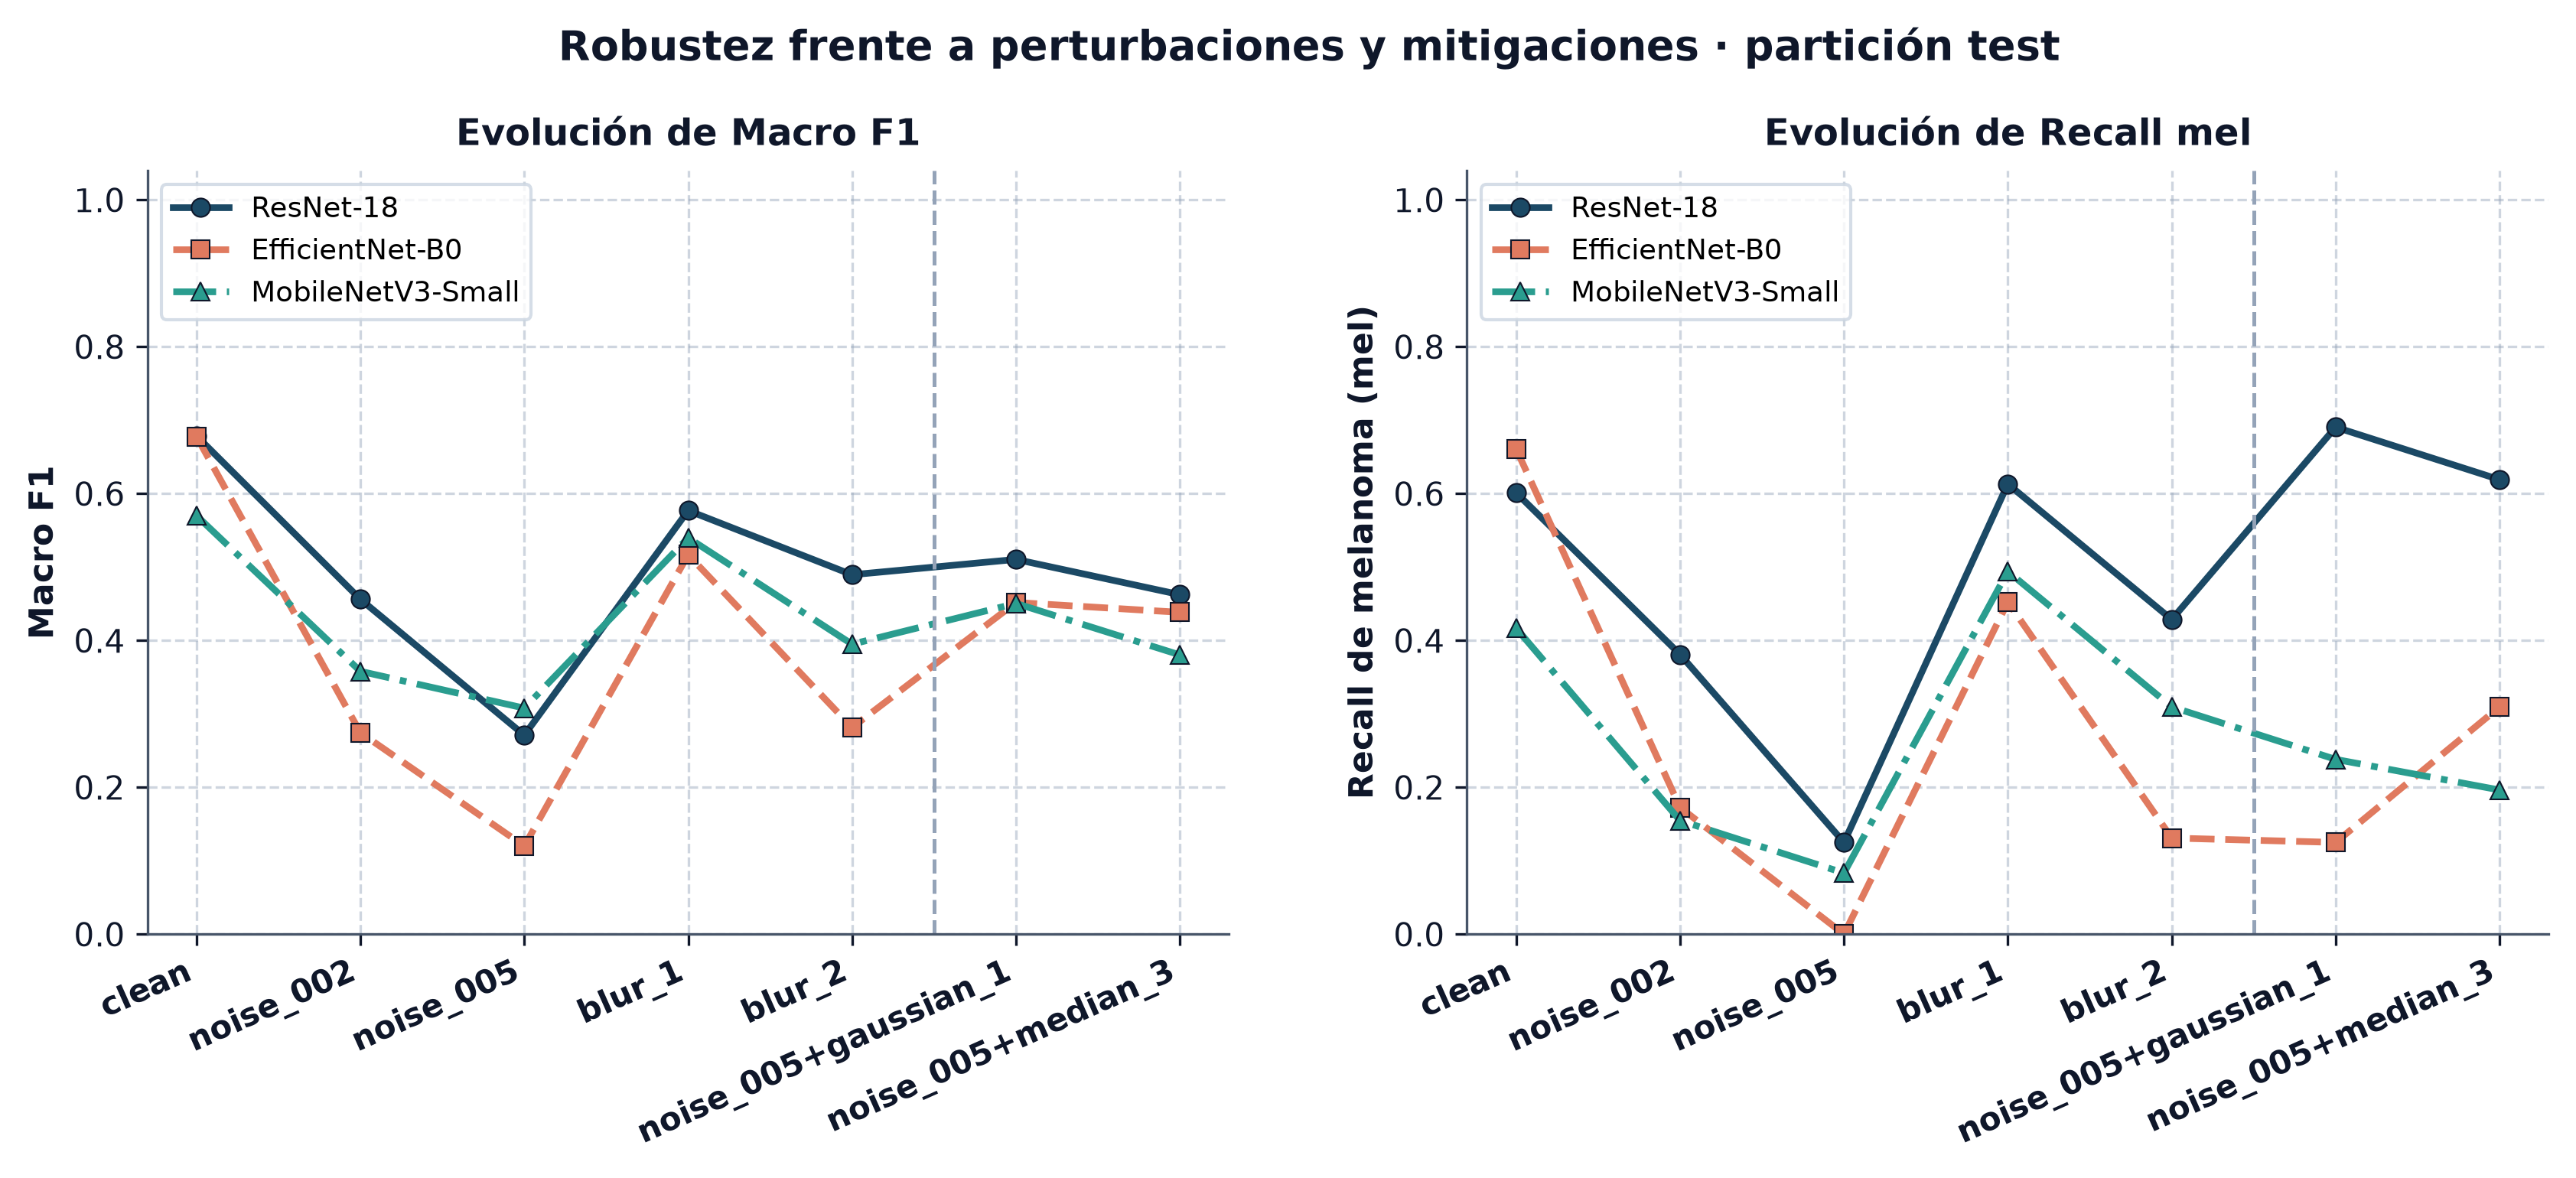
\includegraphics[width=0.76\textwidth]{comparacion_robustez.png}
\caption{Evoluci\'on de Macro~F1 (izquierda) y Recall de melanoma (derecha) en \texttt{test} bajo perturbaciones y mitigaci\'on espacial sobre \texttt{noise\_005}. \texttt{gaussian\_1} aporta $+0.14$ a $+0.33$ pts de Macro~F1 y eleva el Recall \texttt{mel} de ResNet-18 a $0.6905$ (con ca\'ida de precisi\'on $0.5233 \to 0.3648$), evidenciando la mayor fragilidad de EfficientNet-B0 ante ruido.}
\label{fig:comp_robustez}
\end{figure*}

\section{Discusi\'on y Limitaciones}
Los resultados sugieren dos compromisos relevantes entre arquitectura, c\'omputo y robustez. Primero, un menor conteo param\'etrico no garantiza menor latencia en GPU: aunque MobileNetV3-Small posee $7.3\times$ menos par\'ametros y la mitad de VRAM que ResNet-18, su ejecuci\'on \texttt{forward()} a \texttt{batch=1} en GTX~1650 es $3.1\times$ m\'as lenta en limpio ($22.40$ vs.\ $7.22$~ms, con dispersi\'on entre corridas de $15.26\text{--}22.40$~ms frente a $6.86\text{--}9.46$~ms). Como \textbf{hip\'otesis interpretativa} (no verificada mediante perfilado de n\'ucleos CUDA/Nsight), las convoluciones separables y m\'odulos SE inducir\'ian mayor fragmentaci\'on de lanzamientos CUDA y menor intensidad aritm\'etica que los bloques residuales densos $3\times3$ a \texttt{batch=1}; adem\'as, las mediciones reportadas excluyen decodificaci\'on E/S y preprocesamiento/filtrado en CPU. Segundo, como otra \textbf{hip\'otesis interpretativa}, la atenci\'on SE y representaci\'on final $1\,280$-d de EfficientNet-B0 favorecer\'ian la discriminaci\'on fina de melanoma en limpio (Recall $0.6607$, AUC $0.911$), pero con mayor vulnerabilidad ante alteraciones de alta frecuencia como \texttt{noise\_005} ($0.1201$), donde \texttt{+gaussian\_1} no restablece la sensibilidad de melanoma ($0.1250$). De forma an\'aloga, en ResNet-18 la compatibilidad estructural entre bloques residuales y el suavizado \texttt{gaussian\_1} constituye una hip\'otesis plausible del repunte en Recall \texttt{mel} ($0.6905$), aunque a expensas de duplicar los falsos positivos ($92 \to 202$, Prec.\ $0.3648$), confirmando que el prefiltrado es solo una mitigaci\'on parcial.

Persisten limitaciones estructurales del estudio: (1) \texttt{HAM10000\_metadata.csv} identifica lesiones pero no pacientes, pudiendo ubicar distintas lesiones de un mismo individuo en particiones separadas; (2) el dataset proviene de dos centros con predominio de piel clara, limitando la generalizaci\'on externa; (3) la receta \'unica de \texttt{configs/base.json} asegura equidad presupuestaria, aunque no optimiza hiperpar\'ametros individuales; (4) clases minoritarias como \texttt{df} ($n=17$) y \texttt{vasc} ($n=21$) en \texttt{test} presentan alta varianza discreta; (5) la evaluaci\'on se ejecut\'o con una sola semilla (\texttt{seed=42}), y sin superioridad estad\'istica en Macro~F1 entre las dos arquitecturas principales; (6) las verificaciones previas de sesi\'on sobre $\mathrm{RMSE}<4.5$ en miniaturas $16\times 12$ y piloto \texttt{num\_workers=0/4} carecen de artefacto persistido independiente, manteniendo abierta la limitaci\'on de similitud perceptual entre lesiones; y (7) el despliegue interactivo qued\'o excluido por alcance docente.

\section{Conclusiones y Trabajo Futuro}
Se complet\'o de principio a fin el estudio comparativo reproducible entre ResNet-18, EfficientNet-B0 y MobileNetV3-Small sobre HAM10000 bajo partici\'on estratificada por grupos sin fuga y entorno GPU verificado. Sin superioridad ni equivalencia estad\'istica demostrada en Macro~F1 frente a EfficientNet-B0 ($\Delta=0.00084$; IC95\% bootstrap $[-0.0429,+0.0464]$), \textbf{ResNet-18} representa el mejor compromiso observado en este protocolo y GPU: combina el mayor Macro~F1 puntual ($0.6786$), Accuracy ($0.8031$), Bal.\ Acc.\ ($0.7174$) y AUC~OVR ($0.9596$), junto a la menor latencia \texttt{forward()} ($7.22$~ms en limpio; $6.86\text{--}9.46$~ms entre corridas), consumo moderado de VRAM ($434.2$~MiB) y mayor estabilidad ante desenfoque. \textbf{EfficientNet-B0} lidera en Macro~Prec.\ ($0.6741$) y sensibilidad limpia de melanoma ($0.6607$), pero demanda mayor VRAM ($805.7$~MiB), mayor latencia ($22.49\text{--}34.82$~ms) y colapsa ante ruido aditivo. \textbf{MobileNetV3-Small} minimiza VRAM ($211.8$~MiB), pero penaliza el desempe\~no global ($0.5700$) y la latencia GPU ($15.26\text{--}22.40$~ms). Asimismo, el prefiltrado \texttt{gaussian\_1} act\'ua como una \textbf{mitigaci\'on parcial sobre \texttt{noise\_005}} sin reentrenamiento ($+0.14$ a $+0.33$ puntos en Macro~F1), elevando el Recall \texttt{mel} de ResNet-18 a $0.6905$ pero reduciendo su precisi\'on de $0.5233$ a $0.3648$ ($92 \to 202$ falsos positivos).

Como trabajo futuro se proyecta: (1) ejecutar m\'ultiples semillas para cuantificar intervalos de confianza en entrenamiento, (2) validar externamente en colecciones ISIC con mayor diversidad de fototipos, (3) incorporar ruido y desenfoque en el aumento de entrenamiento junto con calibraci\'on de umbrales por clase para endurecer EfficientNet-B0 y controlar falsos positivos, y (4) perfilar operadores CUDA y explorar cuantizaci\'on TensorRT/ONNX para dispositivos embebidos fuera del alcance actual.

\bibliographystyle{IEEEtran}
\bibliography{referencias}
\end{document}
